% Generated by traktat/scripts/sync_latex.py. Edit traktat/tekst/formlaere.txt.
\silentchapter{Proposisjonar}{proposisjonar}
\begin{widebody}\footnotesize
d = definisjon · a = postulat/hypotese · t = modellvilkårsvis følgje · o = observasjon · i = illustrasjon. Desimalnummera viser logiske underordningar, ikkje berre kapittelrekkjefølgje.
\end{widebody}
\vspace{6mm}

\mainprop{1}{d}{Form er ei \hyperlink{kjeldenotat-1}{ordning av skilnader}.}

\prop{1.01}{d}{Å skilje noko ut er å halde noko anna utanfor. Det som då står mellom dei, er ein skilnad.}

\prop{1.011}{t}{Ein skilnad har difor to sider. Han gjev ikkje to uavhengige verder, for kvar side er det ho er, berre mot den andre.}

\prop{1.0111}{i}{Kanten på koppen skil innsida frå utsida. Munnen møter begge ved den same kanten.}

\prop{1.012}{o}{Ein skilnad kan verke før han får eit namn. (Membranen treng ikkje ordet for å halde noko inne.)}

\prop{1.0121}{t}{Å oppdage ein skilnad er difor ikkje å lage han. Ei teikning kan gjere begge delar.}

\prop{1.02}{d}{Skilnader som står i bestemde samanhengar med kvarandre, er ei ordning: kva som er skilt frå kva, og korleis det skilde heng saman.}

\prop{1.021}{t}{Delane i ei ordning er ikkje alltid ferdige før ordninga.

Kvar side av ein skilnad er det ho er mot den andre (1.011). Det som står i ei ordning, kan difor få si bestemming gjennom ordninga.}

\prop{1.0211}{i}{Eit sete bind saman ei bereflate, ein kropp og ei mogleg kvile. Flata kan finnast utan kroppen. Setet kan ikkje forklarast utan kroppen.}

\prop{1.1}{a}{\hyperlink{kjeldenotat-1.1}{Formverda er alt som er tilfelle}: totaliteten av realiserte konfigurasjonar, ikkje av ting.}

\prop{1.11}{d}{Ein konfigurasjon er ei bestemt ordning av bestemde delar (1.02). Han er realisert når han er tilfelle.}

\prop{1.111}{i}{Same treet kan vere stol eller ved.}

\prop{1.12}{t}{Kvar realisert konfigurasjon er bestemt (1.11). Anten er han tilfelle, eller han er det ikkje.

Ingen konfigurasjon er delvis realisert.}

\prop{1.13}{a}{At ein konfigurasjon er nettopp denne, når uendeleg mange andre samanhengar av dei same delane var logisk moglege, har ei forklaring utover konfigurasjonen sjølv.

Forklaringa er det som gjorde nettopp denne meir venteleg enn dei andre.}

\prop{1.131}{t}{Dei same delane kan berre stå i éin samanheng om gongen. Å forklare kvifor nettopp denne vart realisert, er difor å forklare kvifor dei andre ikkje vart det.

Forklaringa ligg i relasjonen mellom den realiserte konfigurasjonen og dei moglege som ikkje vart realiserte.}

\prop{1.2}{d}{Ein konfigurasjonsdel som ikkje vert delt vidare på det \hyperlink{kjeldenotat-1.2}{valde analysenivået}, er eit objekt.

Same objekt kan stå i fleire konfigurasjonar.}

\prop{1.201}{t}{Inndelinga i objekt er eit val av analysenivå.}

\prop{1.2011}{o}{Under nivået held fysikken fram; formgjevinga på nivået gjer det ikkje. (Stolbeinet er udeleleg for snikkaren. For fysikken er det ein konfigurasjon av fibrar, av celler, av molekyl.)}

\prop{1.202}{a}{Kvart objekt er ein konfigurasjon på eit lågare nivå, for under kvart nivå held strukturen fram.

Fysikken er òg eit nivå. Kor langt analysen enn går, finn han difor konfigurasjonar.}

\prop{1.2021}{t}{Ein konfigurasjon er ein samanheng (1.11). Det analysen finn, er difor relasjonar.}

\prop{1.2022}{a}{Ein relasjon krev ledd. Relasjonar mellom relasjonar utan ende er ikkje ein samanheng av noko.}

\prop{1.203}{t}{Det som er ledd og ikkje sjølv relasjon, er substans.

Formverda har difor ein substans. \hyperlink{kjeldenotat-1.203}{Substansen finst uavhengig av kva som er tilfelle}.}

\prop{1.2031}{t}{\hyperlink{kjeldenotat-1.2031}{Utan substans} ville det at ein konfigurasjon er mogleg, avhenge av at ein annan er realisert, og den andre av ein tredje. Regressen stoggar berre i noko som ikkje er konfigurasjon.}

\prop{1.204}{t}{Objektet har ingen delar på nivået sitt (1.2) og difor ingen samanheng som kan skifte der. Det som endrar seg i det, endrar seg på eit lågare nivå (1.202).

Objektet står fast på eitt nivå, substansen på alle. \hyperlink{kjeldenotat-1.204}{Konfigurasjonen er det skiftande}.}

\prop{1.21}{d}{\hyperlink{kjeldenotat-1.21}{Måten objekta heng saman på} i konfigurasjonen, er strukturen til konfigurasjonen.}

\prop{1.211}{i}{Sambandet mellom setet og beinet i ein stol er ikkje ein del til. Delane heng i kvarandre direkte, \hyperlink{kjeldenotat-1.211}{som lenkene i ei kjede}.}

\prop{1.212}{t}{Strukturen er ordninga av skilnadene mellom objekta (1.02). Ordninga seier ikkje kva objekt som står i henne.

Forma til ein konfigurasjon (1) er difor strukturen hans, teken uavhengig av kva objekt som står i konfigurasjonen.}

\prop{1.2121}{t}{To konfigurasjonar med same objekt, men ulik struktur, har ulike former.}

\prop{1.2122}{t}{To konfigurasjonar med ulike objekt, men same struktur, deler form.}

\prop{1.2123}{t}{Forma er difor ikkje sjølv ein konfigurasjon, men \hyperlink{kjeldenotat-1.2123}{moglegheita strukturen har} for å gå att i andre objekt.}

\prop{1.2124}{t}{Ei form utan alternativ (1.131) er ikkje vald, og ho treng inga forklaring. Ho er ei nødvendigheit.}

\prop{1.22}{d}{\hyperlink{kjeldenotat-1.22}{Moglegheita eit objekt har for å inngå i konfigurasjonar}, er valensen til objektet.}

\prop{1.221}{t}{I og med valensane til objekta er \hyperlink{kjeldenotat-1.221}{alle moglege former gjevne}.}

\prop{1.222}{t}{Det moglege er ikkje laga, men gjeve.}

\prop{1.2221}{t}{Ei moglegheit kan ikkje finnast opp, berre avdekkjast.}

\prop{1.2222}{t}{Det moglege ligg fast når nivået er valt. Berre valet av nivå (1.201) er konstruert.}

\prop{1.223}{t}{Valensen høyrer til objektet, og objektet står fast på nivået (1.204). \hyperlink{kjeldenotat-1.223}{Å kjenne objektet fullt ut} ville vere å kjenne alle konfigurasjonane det kan inngå i.

Ei ny moglegheit for eit gjeve objekt kan ikkje oppstå seinare; ei ny skildring av ei moglegheit kan.}

\prop{1.2231}{t}{Kva av det moglege som er realisert, tilgjengeleg og kjent, kan endre seg, ikkje kva som er mogleg.}

\prop{1.23}{t}{Substansen i formverda (1.231, 1.234, 1.2342) er oppleving.}

\prop{1.231}{d}{Ei måling er ein relasjon mellom det som vert målt og det som måler.}

\prop{1.2311}{t}{Det ei måling gjev, er difor ein relasjon, aldri leddet sjølv.}

\prop{1.232}{o}{Fysikken seier alt han seier i storleikar, og kvar storleik er eit utfall av måling eller ein relasjon mellom slike utfall.}

\prop{1.2321}{t}{Fysikken seier difor kva det målte gjer, ikkje kva det er.}

\prop{1.233}{d}{Det som er kjent utan måling, ikkje gjennom ein relasjon, men ved å vere det, er oppleving.}

\prop{1.2331}{o}{Kvar måling er gjeven som oppleving. Det fysikken veit, veit han gjennom opplevinga.}

\prop{1.2332}{d}{Oppleving av opplevinga, opplevinga framstilt på nytt i seg sjølv, er medvit.}

\prop{1.2333}{a}{Oppleving føreset ikkje medvit.}

\prop{1.234}{a}{Når ein natur som er kjend, strekkjer til, har det verkelege ingen natur som ingen kan møte.}

\prop{1.2341}{t}{Opplevinga strekkjer til.

Alt fysikken skil og set i samband, er gjeve som skilnader og samanhengar i henne (1.232, 1.2331). I dei relasjonane fysikken finn, kan ho difor vere ledd.}

\prop{1.2342}{t}{Ein substans som ikkje er oppleving, er ein natur ingen kan møte.

Måling gjev berre relasjonane hans (1.2311), og det som er kjent ved å vere det, er oppleving (1.233). Han forklarer heller ikkje meir enn opplevinga.

Substansen (1.203, 1.234) er difor oppleving.}

\prop{1.2343}{o}{Ein substans som ikkje er oppleving, skapar dessutan ei gåte ingen har løyst: korleis det som ikkje opplever, skulle bli til oppleving.}

\prop{1.235}{d}{Å vere noko er å kjenne det innanfrå. Å kjenne relasjonane noko står i, er å kjenne det utanfrå, å sjå det utanfrå.}

\prop{1.2351}{t}{Fysikken kjenner berre relasjonar (1.2311, 1.2321), og materie er det han skildrar. Materie er difor oppleving, sett utanfrå (1.23): biletet ei oppleving har av ei anna.}

\prop{1.2352}{t}{Materien er ikkje ein annan ting enn opplevinga, og opplevinga er ikkje ein eigenskap ved materien. Biletet og det det er bilete av, er av same substans.}

\prop{1.2353}{t}{Det som vert kjent utanfrå, er relasjonar. Forma er struktur (1.212), og struktur er relasjonar (1.21).

Forma er difor korleis ein del av substansen tek seg ut for ein annan.}

\prop{1.2354}{t}{At materien er oppleving, tyder ikkje at han er min.}

\prop{1.24}{a}{Opplevinga er eitt felt.

Det som vert skilt ut i feltet, er mønster i det, ikkje bitar av det.}

\prop{1.2401}{t}{Ingen del av formverda står difor utanfor relasjon til resten.}

\prop{1.241}{o}{Korleis mange opplevingar kunne bli éi, veit ingen. Men at éi oppleving kan dele seg i fleire som ikkje når kvarandre innanfrå, er kjent.}

\prop{1.242}{t}{Eitt felt som vert avgrensa, krev berre det som er kjent (1.241). Mange som må samlast, krev ei samanslåing ingen kjenner.

Av dei to krev postulatet i 1.24 minst.}

\prop{1.243}{t}{Det som skiftar, er korleis feltet er konfigurert; det som står fast (1.204), er feltet.}

\prop{1.244}{t}{I feltet kan det skiljast ut mønster som ikkje når kvarandre innanfrå (1.241).}

\prop{1.245}{t}{Måten feltet oppfører seg regelmessig på, er naturlovene. Dei vert ikkje lagde på feltet utanfrå, for utanfor feltet finst det inkje.}

\prop{1.2451}{t}{Lovene legg ikkje moglegheiter til valensane (1.221). Dei avgjer kva av det moglege som kan realiserast, og med kva.

Det som kjem til seinare, er materiale og operasjonar lovene kan verke på: tilgang, ikkje moglegheit.}

\prop{1.2452}{d}{Materiell tyder: gjeven ved lovene i feltet, kjend utanfrå.}

\prop{1.2453}{d}{Det som gjeld feltet og lovene i det, same kva nokon veit, er ontologisk. Det som avheng av kva som er kjent om feltet, og av kven, er epistemisk.}

\prop{1.246}{t}{Feltet som heilskap har inkje utanfor seg (1.245). Det kan difor ikkje kjennast utanfrå; det viser seg aldri som ein ting.}

\prop{1.3}{d}{Ei mengd konfigurasjonar som tillèt same operasjonar, er ein klasse.}

\prop{1.31}{d}{Mengda av alle moglege konfigurasjonar i ein klasse er \textit{\hyperlink{kjeldenotat-1.31}{formrommet}} \ensuremath{𝕄}\kjelde{2,10,20} til klassen.}

\prop{1.311}{t}{Formrommet vert ikkje konstruert (1.222), men oppdaga.}

\prop{1.32}{d}{Kvar konfigurasjon i klassen er eitt eksakt punkt i \ensuremath{𝕄}, posisjonen hans. Kvar akse i formrommet er ein målbar eigenskap.}

\prop{1.321}{t}{Eit val av aksar er ein projeksjon av \ensuremath{𝕄}. Forma finst uavhengig av den einskilde målinga, slik eit fjell finst uavhengig av kartet.}

\prop{1.3211}{t}{Fjellet er ikkje i kartet. Men den som les kartet, er av same substans (1.23) som fjellet.}

\prop{1.322}{t}{Det empiriske formrommet er alltid ein slik projeksjon. Sidan strukturen held fram under kvart valt nivå (1.202), fangar inga endeleg mengd parametrar heile den latente kompleksiteten.}

\prop{1.3221}{t}{At det empiriske formrommet er ein projeksjon, tyder ikkje at det er vilkårleg. Somme projeksjonar fangar meir variasjon enn andre.}

\prop{1.323}{t}{Formrommet er eit rom av relasjonar (1.2311). Det viser korleis konfigurasjonane i klassen tek seg ut utanfrå, ikkje kva dei er innanfrå.}

\prop{1.4}{d}{Formrommet deler seg i tre regionar: dei busette, dei forbodne og dei opne.}

\begin{figure}[htbp]\centering
\includegraphics[width=\linewidth]{scan-20261031-p11-busette-opne-forbodne.png}
\caption{Busette, opne og forbodne regionar}
\end{figure}

\prop{1.41}{d}{Dei busette regionane er dei posisjonane som er eller har vore realiserte. Dei utgjer det historiske arkivet.}

\prop{1.411}{a}{Frå det busette vert ny form nådd. Kvar ny realisering tek utgangspunkt i ein busett posisjon og når ein posisjon som grensar til han.

Det busette er ankerpunktet for alt som kjem etter, og den induktive premissen for vidare form.}

\prop{1.412}{o}{Tyngda til ein busett posisjon, kor sterkt han dreg nye realiseringar til seg, veks med kor lenge han har vore busett.}

\prop{1.413}{d}{Totaliteten av busette posisjonar er formhistoria.}

\prop{1.42}{d}{Dei forbodne regionane V er dei ikkje busette posisjonane som er logisk moglege, men utelukka av materielle vilkår.

Dei er utelukka av materialet, strukturen eller energien, slik lovene verkar på det som er for hand.

Forbodet følgjer ikkje regionen, men vilkåra.}

\prop{1.421}{t}{Grensa mellom det forbodne og det opne er ikkje logisk, men materiell, for ho er gjeven ved lovene i feltet (1.2452), brukte på dei materiala og operasjonane som er for hand. (Bøk bøyer seg langs fiberen; granitt gjer det ikkje.)

Vilkåra, ikkje logikken, avgjer kva som er forbode.}

\prop{1.422}{t}{Eit skifte i kva materiale og operasjonar som er for hand, kan opne ein forboden region. At det forbodne er materielt avgrensa, tyder at det tilgjengelege kan vekse; det moglege (1.2231) veks ikkje.}

\prop{1.43}{d}{Dei opne regionane er dei ikkje busette posisjonane som er materielt moglege.}

\prop{1.431}{d}{Ein open region som kan nåast frå det busette utan å gå gjennom det forbodne, er tilgjengeleg.}

\prop{1.4311}{t}{Ein open region som berre grensar til forbodne regionar, er utilgjengeleg (1.411, 1.422) utan materialskifte.}

\prop{1.432}{d}{Dei opne posisjonane som grensar til det busette, er \textit{det \hyperlink{kjeldenotat-1.432}{nærliggande moglege}}\kjelde{59,109}.}

\prop{1.4321}{t}{Det nærliggande moglege er avgrensa. Det ligg spent ut mellom det busette på den eine sida og det forbodne og dei opne regionane lenger ute (1.431, 1.4311) på den andre.}

\prop{1.5}{d}{Ved sida av den materielle delinga går ei \hyperlink{kjeldenotat-1.5}{epistemisk}\kjelde{16,17}.

Ho gjeld alltid relativt til det nokon på eit gjeve tidspunkt veit og har tenkt, ein kunnskapsstand.

Dei posisjonane ein veit verkar eller sviktar, er det kjende K; dei ein veit verkar, er K+.

Dei posisjonane som er tenkte, men ikkje avgjorde, er det tenkjelege C.

Resten, U = \ensuremath{𝕄} \ensuremath{∖} (K \ensuremath{∪} C), er det utenkjelege.

K og C har inkje felles. Partisjonen er \ensuremath{Π} = (K, C, U).}

\prop{1.501}{d}{C kallar eg tankerommet, K kunnskapsrommet. Rørsla i og mellom dei, medan ho går gjennom dei materielle regionane, er formgjeving.}

\prop{1.51}{t}{Dei to delingane fell ikkje saman.

Ein forboden region kan vere tenkt: materielt utelukka, men tenkt.

Ein open region kan vere utenkjeleg: materielt mogleg, men utanfor det nokon har tenkt.}

\prop{1.511}{t}{Begge delingane trengst difor i ei skildring av formverda. Den materielle delinga seier kva vilkåra tillèt, den epistemiske kva som er kjent og tenkt.}

\prop{1.512}{t}{Grensene i den epistemiske delinga er epistemiske, ikkje ontologiske (1.2453). Dei flyttar seg når kunnskapen flyttar seg, medan det moglege (1.2231) står fast.}

\prop{1.52}{a}{Det ein veit verkar eller sviktar, er kjent fordi det er prøvd i ein realisert konfigurasjon.

Det busette avgjer difor K. K rommar både suksessar og fiaskoar.

Formhistoria avgjer kva som er kjent mogleg.}

\prop{1.53}{t}{\hyperlink{kjeldenotat-1.53}{Grensa mellom C og U kan ikkje sjåast frå C}. Ein kan ikkje vite kva ein ikkje kan tenkje.}

\prop{1.531}{t}{Innanfrå kan U nemnast som komplement, men inkje element i U kan nemnast. Eit element i U kan berre peikast ut frå ein vidare kunnskapsstand, og der er det ikkje lenger utenkjeleg.}

\prop{1.54}{t}{Ei rørsle tek utgangspunkt i C eller K og legg noko til C eller K. Det gjev \hyperlink{kjeldenotat-1.54}{fire retningar}\kjelde{16,17}:

C\ensuremath{→}C (konseptekspansjon) · Innanfor C · Utviding: C veks\\
C\ensuremath{→}K (konjektur \ensuremath{→} kunnskap) · Frå C til K · Kollaps: ei tenkt form vert avgjord\\
K\ensuremath{→}C (kunnskap \ensuremath{→} konjektur) · Frå K til C · Opning: det kjende opnar nye konjekturar\\
K\ensuremath{→}K (kunnskapsutdjuping) · Innanfor K · Oppløysingsauke: det kjende vert finare}

\begin{figure}[htbp]\centering
\includegraphics[width=\linewidth]{scan-20261031-p13-c-k-operator-tabell-og-rorsle.png}
\caption{C–K-operasjonane}
\end{figure}

\prop{1.541}{t}{Tanken veks innanfrå: frå det tenkte (C\ensuremath{→}C) eller frå det kjende (K\ensuremath{→}C). Det som kjem inn frå U, kjem ikkje ved at nokon ser over grensa (1.53).}

\prop{1.55}{d}{Den delen av C som ligg i det nærliggande moglege, er fronten: tilgjengeleg og tenkt, men ikkje kjend. Der kan det tenkte prøvast (1.52) og bli kjent.}

\prop{1.6}{d}{Konfigurasjonar lukka under sum, differanse og produkt, og under transformasjonar \ensuremath{θ}, med delrelasjonen \ensuremath{≤}, utgjer ein \textit{\hyperlink{kjeldenotat-1.6}{formalgebra}}\kjelde{11,18}.}

\prop{1.61}{d}{I formalgebraen utfører formgrammatikken diskrete overgangar.

Reglane slår til ved \textit{\hyperlink{kjeldenotat-1.61}{innleiring}}\kjelde{18}, når ei delform vert kjend att inne i heilforma. Inndatageometrien er einaste premiss.

Ein formgrammatikk er eit trippel SG = (S, R, s\ensuremath{₀}): ei mengd posisjonar S \ensuremath{⊆} \ensuremath{𝕄}, tekne ved forma si (1.212), reglar R = \{a\ensuremath{ᵣ} \ensuremath{→} b\ensuremath{ᵣ}\} og ei startform s\ensuremath{₀}. Reglane transformerer former:

Regelbruk · s \ensuremath{→} (s \ensuremath{−} \ensuremath{θ}(a\ensuremath{ᵣ})) + \ensuremath{θ}(b\ensuremath{ᵣ}) når \ensuremath{θ}(a\ensuremath{ᵣ}) \ensuremath{≤} s · Finn delforma; byt henne ut\\
Språk · L(SG) = \{s \ensuremath{∈} S: s\ensuremath{₀} \ensuremath{→}* s\} · Alle former grammatikken kan generere\\
Utløysing · \ensuremath{θ}(a\ensuremath{ᵣ}) \ensuremath{≤} s · Kvar innleiring gjev eitt mogleg steg; eitt av dei vert teke\\
Premiss · Noverande geometri, ikkje konstruksjonshistorie}

\prop{1.611}{t}{Formalgebraen ser gjennom det valde nivået, der objekta er atom. Der delane er liner, flater og lekamar, har algebraen ingen atom, og \hyperlink{kjeldenotat-1.611}{innleiringa} finn delformer som inga objektdeling gav på førehand (1.223).}

\prop{1.62}{t}{Den fullstendige grammatikken er regelforma til valensane (1.22) og ligg fast med dei (1.223).

Den delen av han som er kjend og i bruk, er ein historisk grammatikk. Han veks når det kjende veks, medan det moglege (1.2231) står fast.

Med SG meiner eg heretter ein historisk grammatikk. Språket hans er den delen av formrommet som kan nåast frå startforma.

Eitt regelbruk er eitt steg. Det nærliggande moglege (1.432) ligg eitt steg frå det busette.}

\prop{1.63}{t}{Ein grammatikkoperasjon endar i C. Han gjer altså moglegheiter tenkte, frå ei tenkt form (C\ensuremath{→}C) eller frå ei kjend (K\ensuremath{→}C).

Realisering er ein C\ensuremath{→}K-operasjon: ho avgjer konfigurasjonen.}

\mainprop{2}{t}{Ikkje alle posisjonar er like sannsynlege.}

\prop{2.01}{t}{Forbodet (1.42) skil ut det som ikkje kan vere, men lèt mange posisjonar stå opne (1.43).

Var alle dei opne like sannsynlege, ville ingen relasjon til dei urealiserte gjere den realiserte meir venteleg enn dei. Realiseringa ville vere eit lotteri, og forklaringa som 1.13 set, ville ikkje finnast.}

\prop{2.011}{o}{Dei busette posisjonane ligg ikkje jamt spreidde over det materielt moglege. Tradisjonar som aldri har møtt kvarandre, kjem fram til same form.}

\prop{2.02}{t}{Forklaringa av ein konfigurasjon gjer han meir venteleg enn dei andre (1.13). Noko verkar difor på fordelinga.}

\prop{2.021}{t}{Det som verkar, skuvar ikkje den einskilde forma, for ho er realisert eller ikkje (1.12). Det verkar på fordelinga, og der forma elles kunne ha vore, tynner det altså ut sannsynet.}

\prop{2.1}{d}{Det som endrar sannsynsfordelinga over det som ikkje er forbode, er eit seleksjonstrykk\kjelde{3}.

Trykket er ikkje ein regel, men ein gradient. Det gjer somme posisjonar mindre sannsynlege enn andre, utan å forby dei.

Det utelukkar ved å tynne ut.}

\prop{2.101}{t}{Forma er det som \hyperlink{kjeldenotat-2.101}{står att} når trykka har utelukka alt anna\kjelde{15,77,78}.}

\prop{2.11}{t}{Eit trykk som inkje tynner ut, er inkje trykk. Eit trykk som tynner ut alt unnateke éin region til inkje, er ikkje lenger eit trykk, men determinisme.}

\prop{2.111}{t}{Berre mellom nulltrykket og determinismen finst alternativ som trykka gjer ulikt sannsynlege (2.01, 1.2124).

Mellom dei to ligg heile rommet for design.}

\prop{2.112}{o}{Mellom dei to grensene ligg alle observerte trykk, for ingen observert formklasse er utan trykk, og ingen er fullt determinert.}

\prop{2.12}{a}{Fleire seleksjonstrykk verkar samstundes, kvart for seg.}

\prop{2.121}{t}{Verka berre eitt trykk, ville det ikkje finnast avvegingar. All variasjon ville vere variasjon i kor nær forma kom det eine, ikkje i kva ho vog mellom.}

\prop{2.122}{t}{Eit trykk som er likt over alle observerte tilfelle, er latent. Det verkar framleis, men berre variasjon i vilkåra kan påvise trykket.}

\prop{2.13}{a}{I kvar realisert posisjon peikar minst to trykk i motstridande retningar, for inga form er best for alle trykk samstundes.}

\prop{2.131}{t}{Kvar realisert form er difor eit kompromiss, der minst eitt trykk ikkje er fullt forløyst.}

\prop{2.1311}{t}{Utan eit spesifikt trykksett er omgrepet «suboptimal» tomt. Omgrepet føreset ein referanse.}

\prop{2.14}{d}{Den delte moglegheita for operasjonar som avgrensar ein klasse (1.3), er klassen sin \hyperlink{kjeldenotat-2.14}{affordansestruktur}\kjelde{12,55,56}.}

\prop{2.141}{t}{Affordansestrukturen er konstant innanfor klassen, og ein konstant kan ikkje forklare ein skilnad. Han kan seie kvar formene samlar seg og kor trongt, men det klassen er til for, seier ingenting om kvifor formene i han er ulike.}

\prop{2.15}{t}{Det som forklarer, er trykka (1.131, 2.1). Den projeksjonen av formrommet som forklarer best (1.3221), er den som gjer flest seleksjonstrykk synlege.}

\prop{2.2}{d}{Materialaffordansen er operasjonane materialet tillèt og hindrar\kjelde{12}.

Utover forbodet i 1.42 er han ikkje ein regel, men ein gradient. Han bind sannsynsfordelinga utan å tvinge geometrien (2.1).

Signaturen hans i forma er latent (2.122) der alle tilfella har same materiale.}

\prop{2.201}{o}{Formhistoria er systematisk langsamare enn materialhistoria. Stål fanst i hundreår før stålrøyrstolen\kjelde{54}.

Først mangla operasjonen, og regionen var forboden (1.422). Så kom operasjonen, og regionen låg open, men ikkje tenkt (1.51).

Røyret låg i sykkelfabrikken i eit halvt hundreår. Nokon måtte sjå stolen i røyret.}

\prop{2.2011}{i}{Stolen låg i røyret som ei delform (1.611) ingen hadde skilt ut.}

\prop{2.202}{a}{\hyperlink{kjeldenotat-2.202}{Stil kan predikere} formvariasjon betre enn materiale åleine.}

\prop{2.2021}{t}{Materialet set difor rammene, ikkje utfallet (2.2). Variasjonen vert boren av mange trykk (2.121, 2.13) på ein gong.}

\prop{2.21}{t}{Materialaffordansen er eitt trykk mellom mange.

Ein samlevariabel som tek opp i seg mange samtidige trykk, kan predikere formvariasjon betre enn kvart einskildtrykk. Stilperioden (2.202, 2.2021) er ein kandidat til ein slik samlevariabel.}

\prop{2.211}{t}{Som samlevariabel er stilen eit aggregat som tek opp mange samtidige trykk i éin etikett, inga forklaring.}

\prop{2.212}{t}{Stilen er ikkje ei sjølvstendig årsak, men eit symptom på trykka.}

\begin{figure}[htbp]\centering
\includegraphics[width=\linewidth]{scan-20261031-p16-royrstol-utvikling.png}
\caption{Frå sykkelramme til røyrstol}
\end{figure}

\mainprop{3}{t}{Seleksjonstrykka spenner ut eit landskap over formrommet.}

\prop{3.01}{t}{Kvart seleksjonstrykk endrar sannsynet for kvar posisjon med ein positiv faktor (2.1): det tynner ut, men forbyr ikkje. Verkar trykka kvart for seg (2.12), vert faktorane gonga saman, og logaritmen av eit produkt er ein sum.

Den samla verknaden i kvar posisjon er difor éin storleik. Han er gjeven opp til eit fast tillegg, og berre skilnader i han tel.}

\prop{3.1}{d}{\textit{\hyperlink{kjeldenotat-3.1}{Tilpassingslandskapet}} \ensuremath{Λ}\kjelde{3,8,58} er det dei verksame seleksjonstrykka legg over formrommet når dei verkar samstundes.

Kvar posisjon held ein verdi: kor mykje av trykka som står uforløyst der. Verdien er spenninga i posisjonen.

Di lågare spenninga, di meir sannsynleg er posisjonen.

Formelt. \ensuremath{Λ}(x, t) = \ensuremath{Σ}j \ensuremath{λ}j (x, t), der \ensuremath{λ}j er minus logaritmen av faktoren trykket j legg på sannsynet for x. Trykket sjølv er \ensuremath{−}\ensuremath{∇}\ensuremath{λ}j: retninga der forma vert meir sannsynleg, ikkje ei kraft på henne (2.021). Summen av trykka er \ensuremath{−}\ensuremath{∇}\ensuremath{Λ}. Der aksane er diskrete, står \ensuremath{∇} for skilnaden over eitt steg. Låg spenning er god tilpassing; sannsynet samlar seg i dalane.}

\prop{3.11}{t}{Landskapet lèt seg utanfrå berre lodde i ettertid, gjennom det som er prøvd (1.52). Det målte ber likevel framover, lokalt.}

\prop{3.12}{a}{Trykk som strir mot kvarandre (2.13), kan ikkje møtast fullt ut i same posisjon, og same kompromiss kan nåast på fleire måtar. Landskapet har difor mange lokale minimum.}

\prop{3.121}{d}{Ein dal er staden der kvart steg bort kostar; ryggane er tilstandane sannsynet skyr. Dalane er landskapet sine attraktorar.}

\prop{3.122}{t}{At landskapet har fleire dalar (3.12), tyder ikkje at éin av dei er best langs alle aksar. Modellen føreset inga eine fullkomne form.}

\prop{3.2}{d}{Stabiliteten til ein dal svarar til djupna og brattleiken på dalveggane.

Bratte veggar gjev \textit{\hyperlink{kjeldenotat-3.2}{kanalisering}}\kjelde{8}: forma støyter forstyrringar frå seg.}

\prop{3.21}{t}{Djupe, bratte kanalar fryser dimensjonane; slake rommar fluktuasjonen.}

\prop{3.3}{d}{Formene si sverming kring eit felles tyngdepunkt i landskapet er ein \textit{stilart}\kjelde{9,53}.

Stilarten er ikkje ein kategori, men ein sverm.

Stilperiodar er ikkje øyar. Dei går gradvis over i kvarandre.

(Ingen har nokon gong sett ein stil. Ein ser stolar som liknar kvarandre.)}

\prop{3.31}{t}{Kvar stol er eksakt (1.12); svermen er det ikkje. Grensene hans er difor naudsynleg uskarpe.

Det 2.211 fann som aggregat i statistikken, er ein sverm i landskapet.}

\prop{3.4}{a}{Formgjevinga skapar ikkje grunnstrukturen i landskapet.

Han følgjer av vilkår formgjevinga ikkje rår over: materielle, energetiske og dei behova formene skal møte.

Men kvar realisert form er sjølv eit vilkår for den neste. Ho tek plass, bind stoff, går inn i andre konfigurasjonar og gjer det busette tyngre (1.412).

Kvar realisering endrar difor landskapet lokalt.}

\prop{3.41}{t}{I landskapet finn isolerte tradisjonar den same dalen utan å utveksle eit ord (2.011). Uavhengig konvergens stadfestar at attraktoren ikkje er konvensjonell, men reell.}

\prop{3.411}{d}{Reell tyder her: gjeven ved vilkåra i 3.4, lovene i feltet og dei behova formene skal møte, same kva tradisjon som navigerer.}

\mainprop{4}{t}{Landskapet er dynamisk.}

\prop{4.01}{t}{Kvar realisering endrar landskapet (3.4). Så lenge noko vert realisert, står landskapet ikkje stille.}

\prop{4.1}{a}{Seleksjonstrykka kviler aldri.

Dalar djupnar, grunnar, flyttar seg, deler seg, smeltar saman.

Optimal tilpassing er lokal i tid.}

\prop{4.11}{o}{Ein ny teknologi flyttar grensa for det forbodne; ein ny marknad endrar kva landskapet løner; eit nytt materiale utvidar operasjonsrommet.}

\prop{4.12}{t}{Gradvise trykkforskyvingar kan hope seg opp til ein dal forsvinn. Landskapet endrar seg jamt; staden for minimumet gjer eit sprang.

Ein slik overgang er ein bifurkasjon.}

\prop{4.2}{o}{Lange periodar med stillstand bryt saman i brå skifte: radiasjon inn i ein ny region, deretter konvergens.}

\prop{4.21}{t}{Det brå spranget er difor merket etter ein jamn dynamikk, ikkje eit brot med han, når vilkåra endrar seg jamt (4.12). Siktlinja (3.11) er lang i stillstanden og brotnar i bifurkasjonen.}

\prop{4.3}{t}{Landskapet har minne.

Kvar realisert form endrar trykka for den neste (3.4), og kvar ny form tek utgangspunkt i ein busett posisjon (1.411). All formgjeving er difor omformgjeving: kvar ny form arvar eit landskap og ein posisjon.

\textit{\hyperlink{kjeldenotat-4.3}{Stiavhengigheit}}\kjelde{14} er eit grunntrekk, ingen anomali.}

\prop{4.4}{o}{Med kvar realisering flyttar \textit{det nærliggande moglege}\kjelde{59,109} (1.432) seg.

\hyperlink{kjeldenotat-4.4}{Materialstraumane} driv landskapsendringa\kjelde{79}. Dei flyttar grensa for det forbodne, og med henne det nærliggande moglege (1.422).

Det tilgjengelege formrommet veks i hovudsak kumulativt.}

\prop{4.41}{t}{Det tilgjengelege kan vekse; det moglege (1.2231) veks ikkje.}

\prop{4.5}{t}{Når eitt trykk dominerer, samlar fordelinga seg om éin attraktor (3.1).

Eit eineveldande trykk nærmar seg determinismen (2.11). Det forklarer ikkje form, men er fråværet av forklaring (1.2124).

Mangfald (2.121) speglar mangfald av aktive trykk.}

\mainprop{5}{t}{Formverda rommar agentar som svarar på landskapet.}

\prop{5.01}{t}{Eit landskap flyttar ingenting (2.021, 3.1).

Det endrar sannsynet for at ein posisjon vert realisert, og verkar difor berre gjennom det som realiserer, i den mon det følgjer gradienten.}

\prop{5.011}{t}{Når ein formtype vert laga på nytt i eit landskap som endrar seg (4), går han att berre om det som lagar han, svarar på endringa. Elles vert han ført med og omforma.

Objekta står fast (1.204), men samanhengen mellom dei må haldast. (Ein stein held seg derimot utan å svare; det er lovene i feltet som held steinen.)}

\prop{5.012}{i}{Tenk ein formtype som held seg gjennom skiftande vilkår: ei setehøgd som går att, medan kvar stol vert laga på nytt. Skal typen halde seg når vilkåra endrar seg, må noko svare.}

\prop{5.013}{t}{Å svare er å ta noko inn og gje noko ut. Det som svarar, har difor eit indre og eit ytre, og ei grense der dei møtest.}

\prop{5.02}{d}{\hyperlink{kjeldenotat-5.02}{Ei hinne} er ei mengd tilstandar som skil eit indre frå eit ytre, slik at det indre og det ytre er uavhengige av kvarandre når desse tilstandane er gjevne (1.011)\kjelde{83}. Gjennom hinna går observasjonane inn og handlingane ut.}

\prop{5.021}{d}{Ei hinne er sjølvhalden i den grad verksemda i det indre held henne oppe. Ei grense som berre den som analyserer, teiknar (1.201), kallar eg ei analysegrense.}

\prop{5.022}{d}{Eit sjølv er eit mønster i feltet (1.244), avgrensa av ei sjølvhalden hinne.}

\prop{5.0221}{o}{Hinner vert haldne i ulik grad: nokre av det indre, nokre av andre, dei fleste av begge.}

\prop{5.0222}{t}{Å vere eit sjølv er difor ein grad (5.021).}

\prop{5.023}{t}{Steinen er ikkje eit sjølv.

Han held seg, men det er lovene i feltet som held grensa hans (1.245), ikkje verksemd i det indre. Hinna hans er ikkje sjølvhalden (5.021).}

\prop{5.024}{t}{Innanfrå er sjølvet ei oppleving som ikkje når inn i andre mønster i feltet (1.244). Det ho har av resten, er tilstandane i hinna (5.02).

Utanfrå (1.235) er sjølvet hinna og det ho held.}

\prop{5.025}{t}{Det sjølvet har av det ytre, er tilstandane i hinna. Det ser difor ikkje feltet, men ei koding av feltet på hinna.

Persepsjonen er ikkje eit vindauge, men eit grensesnitt.}

\prop{5.0251}{t}{Sjølvet kan ikkje halde kodinga opp mot det ho kodar, for det har berre kodinga.

Det som held kodinga oppe, er difor ikkje at ho liknar, men at ho held hinna (5.021). Kodinga viser det sjølvet treng for å halde seg.}

\prop{5.026}{t}{Fleire sjølv i same felt har eit felles ytre, alt som ligg utanfor dei alle. Dei deler difor éi verd, sjølv om kvart har si eiga koding av henne.

Uavhengig konvergens (3.41) er spor av den verda dei deler.}

\prop{5.027}{t}{Det eit sjølv vil, er innanfor hinna. Det verkar utover berre gjennom hinna, som handling. (Ønske rører ikkje fjellet; ei hand kan.)}

\prop{5.028}{t}{Kroppen til eit sjølv er korleis ei avgrensa oppleving tek seg ut utanfrå (5.024, 1.2351).

Biletet følgjer det det er bilete av, og lagar det ikkje.}

\prop{5.0281}{o}{Den delen av biletet som følgjer opplevinga tettast, er hjernen.}

\prop{5.1}{a}{Landskapet til kvar klasse vert navigert av minst eitt system via \hyperlink{kjeldenotat-5.1}{negativ tilbakekopling}.}

\prop{5.11}{d}{Eit system som held avviket mellom forventing og møte under ein terskel, er ein agent.

Formelt er A = (m, \ensuremath{π}, \ensuremath{ε}).

m er ein \textit{\hyperlink{kjeldenotat-5.11}{generativ modell}}\kjelde{19,21,83,84} over ei delmengd av aksane i formrommet. Han ber òg det agenten føretrekkjer å møte, målregionen hans.

\ensuremath{π}\textsubscript{A} er politikken som minimerer variasjonell fri energi mellom det m predikerer og det agenten observerer gjennom hinna.

\ensuremath{ε} er toleransen for divergensen mellom prediksjon og observasjon.

Agens krev berre denne strukturen, ikkje medvit (1.2332), intensjon eller nervesystem.

Formelt. D\textsubscript{k}(t; \ensuremath{π}) er divergensen langs aksen X\textsubscript{k}, t fram i tid, og D\textsubscript{k}(\ensuremath{π}) = D\textsubscript{k}(0; \ensuremath{π}). \ensuremath{𝒫}\textsubscript{A} er politikkane A kan ta i bruk. F[m, \ensuremath{π}] er den variasjonelle frie energien: eit tak over overraskinga ved det agenten observerer.

D\textsubscript{k}(t; \ensuremath{π}) = D\textsubscript{KL}(p\textsubscript{obs}(x\textsubscript{k}, t) \ensuremath{∥} p\textsubscript{m,\ensuremath{π}}(x\textsubscript{k}, t)) · Divergensen langs X\textsubscript{k}\\
D\textsubscript{k}(\ensuremath{π}\textsubscript{A}) \ensuremath{≤} \ensuremath{ε} for minst éin X\textsubscript{k} · Agenten held noko innanfor toleransen\\
\ensuremath{π}\textsubscript{A} = arg min\textsubscript{\ensuremath{π}\ensuremath{′} \ensuremath{∈} \ensuremath{𝒫}\textsubscript{A}} F[m, \ensuremath{π}\ensuremath{′}] · Politikken minimerer fri energi\\
\ensuremath{τ}\textsubscript{k}(A) = sup\{t \ensuremath{≥} 0: det finst \ensuremath{π} \ensuremath{∈} \ensuremath{𝒫}\textsubscript{A} med D\textsubscript{k}(t\ensuremath{′}; \ensuremath{π}) \ensuremath{≤} \ensuremath{ε} for alle 0 \ensuremath{≤} t\ensuremath{′} \ensuremath{≤} t\} · Horisonten langs X\textsubscript{k}; null når mengda er tom}

\prop{5.111}{t}{Definisjonen er uavhengig av kva agenten er laga av\kjelde{88,89}. Eit kvart system som oppfyller vilkåra, er ein agent.}

\prop{5.1111}{i}{Biologisk vev navigerer via bioelektrisk polarisering\kjelde{22,24,85}; menneskeleg praksis via materiell friksjon; ein slimsopp via oscillerande samandragingar; ein språkmodell via vektoriell merksemd.}

\prop{5.112}{t}{Fri energi er eit tak over overraskinga, og den venta overraskinga er uvissa i det møtte pluss divergensen. Den som held taket lågt, held òg divergensen låg.

Men at politikken held taket så lågt han kan, sikrar ikkje at divergensen kjem under \ensuremath{ε}.

Toleransen er eit eige krav.}

\prop{5.113}{t}{Eit system med \hyperlink{kjeldenotat-5.113}{negativ tilbakekopling} (5.1) er ein slik agent.

Den eldre kybernetiske forma (mål, avvik, justering)\kjelde{4,5,7} er eit spesialtilfelle: målet er eit smalt band kring éin konfigurasjon g, avviket divergensen frå bandet, og justeringa politikkoppdateringa. (Termostaten har bandet i hysteresen til brytaren.)

Fleire tradisjonar har funne same strukturen kvar for seg.

Formelt. Krympar bandet til eit punkt \ensuremath{δ}g, veks divergensen i 5.11 mot det uendelege så snart det møtte spreier seg. Berre den omvende er endeleg: DKL (\ensuremath{δ}g \ensuremath{∥} pobs ) = \ensuremath{−}ln pobs (g), kor uventa målet er under det agenten møter. Den reine punktforma er grensa for 5.11, ikkje eit tilfelle av henne.}

\prop{5.114}{d}{Prediksjonshorisonten \ensuremath{τ}k (A) er kor langt fram A, med ein politikk han kan ta i bruk, kan halde divergensen langs Xk under \ensuremath{ε}. Horisonten til agenten, \ensuremath{τ}(A), er den lengste av prediksjonshorisontane.}

\prop{5.1141}{a}{Ein realisert modell har endeleg mange parametrar.}

\prop{5.1142}{t}{Horisonten er endeleg for alle realiserte agentar.

Ein endeleg modell fangar ikkje heile den latente kompleksiteten (1.322), landskapet kviler aldri (4.1), og somme endringar er brå (4.12). Langs kvar akse skil det observerte seg difor før eller seinare frå det predikerte meir enn \ensuremath{ε}.}

\prop{5.115}{t}{Eit sjølv, sett utanfrå, er ein agent som held si eiga hinne.

Hinna finst berre så lenge tilstandane hennar held seg innanfor ei avgrensa mengd (5.02). Den som held henne oppe frå det indre (5.021), held avviket mellom den venta mengda og det som vert møtt, under ein terskel.

Det er det 5.11 krev.}

\prop{5.116}{t}{Ikkje kvar agent er eit sjølv.

Termostaten held ein temperatur, men hinna hans vert halden av nokon annan: han vert bygd og halden ved like utanfrå.

Han er ein agent, ikkje eit sjølv.}

\prop{5.117}{t}{Strukturen legg ikkje oppleving til. Det strukturen er bilete av (1.2351), er opplevinga.}

\prop{5.118}{t}{Den som veit og har tenkt i 1.5, er ein agent. Kunnskapsstanden er alltid kunnskapsstanden til nokon som navigerer.}

\prop{5.12}{o}{Agens er stratifisert: strukturen er stabil, oppløysinga varierer.}

\prop{5.121}{i}{Termostaten: eitt mål, éin dimensjon, éin brytar.}

\prop{5.122}{i}{Treet: fleire gradientar, ingen sentral prosessor. Kvar grein navigerer lokalt.}

\prop{5.123}{i}{Kolonien: millionar av agentar. Reiret trer fram i feltet mellom agentane.}

\prop{5.124}{i}{Pattedyret: prediksjon, minne, planlegging\kjelde{64,65}. Representasjonen strekkjer seg over tid.}

\prop{5.125}{i}{Den som formgjev for andre: representasjonen strekkjer seg forbi behova til agenten sjølv, til dei som skal leve med forma.}

\begin{figure}[htbp]\centering
\includegraphics[width=\linewidth]{scan-20261031-p21-agentrang.png}
\caption{Agens frå termostat til designar}
\end{figure}

\prop{5.13}{a}{Det agenten føretrekkjer å møte, er låg spenning i posisjonen langs aksane modellen dekkjer (3.1). Å halde divergensen nede er då å følgje gradienten nedover.

Agenten svarar på gradienten slik han når agenten gjennom hinna (5.025), ikkje på forma\kjelde{63,64}.}

\prop{5.131}{t}{Agenten finn ikkje opp målet, for målet er ein region i eit rom som er gjeve (1.222). Det som er hans, er at han held målet.}

\prop{5.132}{t}{Navigasjon krev berre den lokale gradienten\kjelde{63}. Lokale steg gjev global form, utan at nokon ser forma.}

\prop{5.14}{d}{Spenninga i 3.1 ligg over formrommet. Den indre spenninga \ensuremath{σ}k (A) er avstanden langs Xk mellom det agenten møter og målregionen hans, slik han verkar inne i agenten. Ho set politikken i rørsle.}

\prop{5.141}{t}{Indre spenning kjem frå minst tre stader: verda mot målregionen, sansinga mot forventinga, og målet langs éin akse mot målet langs ein annan. Den første er landskapet (3.1, 5.13), den andre divergensen (5.11), den tredje kompromisset (2.13).}

\prop{5.142}{o}{Spenninga i ein bjelke, over hinna til ei celle og i eit menneske er same slag storleik, avvik frå ein føretrekt tilstand som driv ei rørsle attende mot han. Berre der ein politikk (5.11) tek imot spenninga, set ho arbeid i gang.}

\prop{5.143}{t}{Ein agent utan indre spenning langs ein akse har anten nådd målet langs aksen eller mista det.}

\prop{5.144}{a}{Innanfrå er indre spenning kjend som uro når divergensen langs aksen står over toleransen; når han fell attende under, er ho kjend som ro.}

\prop{5.1441}{o}{Svolt, smerte og frykt følgjer trugsmål mot det ein organisme må halde. Metting, lindring og tryggleik følgjer at trugsmålet fell bort.}

\prop{5.15}{d}{Evna til å nå same målregion frå ulike utgangspunkt og på ulike vegar er \textit{\hyperlink{kjeldenotat-5.15}{kompetanse}}\kjelde{21}.}

\prop{5.151}{t}{Kompetansen syner seg berre under forstyrring. Ein kompetent agent når same mål på ein annan veg når vegen vert sperra; ein refleks kjenner berre éin.}

\prop{5.152}{d}{\hyperlink{kjeldenotat-5.152}{Kompetansen kan teljast}.

Talet på storleiksordenar av steg politikken sparar samanlikna med blind leiting mot målet G, er

\formel{ν(A; G) = \log_{10}(E N_{blind}(G) / E N_{A}(G))}

med forventingane tekne over utgangspunkt og forstyrringar, og rekna der begge er endelege. \ensuremath{ν} = 0 er inga betring på blind leiting; \ensuremath{ν} < 0 er verre; \ensuremath{ν} > 0 er kompetanse.}

\prop{5.153}{t}{Kvar måling av kompetanse er gjord av ein observatør, i eit rom observatøren har valt (1.321). Målinga seier difor ikkje berre noko om agenten, men òg om observatøren.}

\prop{5.2}{d}{At avvik ikkje er likegyldige for agenten, er \hyperlink{kjeldenotat-5.2}{omhug} \ensuremath{ω}(A)\kjelde{23,68}.

For kvar akse Xk er \ensuremath{ω}k (A) kor mykje arbeid ei eining indre spenning langs Xk set i gang i politikken.

Omhug er ikkje eit tal, men ein profil over aksane.}

\prop{5.201}{t}{Omhug vert målt i arbeid, ikkje i kunnskap.

Ein agent kan predikere ein akse fullkome og ikkje røre seg for han, for kunnskap utan omhug predikerer, men endrar ikkje.

Omhugen set i gang arbeidet, både det som måler og det som endrar.}

\prop{5.21}{d}{\hyperlink{kjeldenotat-5.21}{Kapasiteten} \ensuremath{κ}(A) er dei aksane der A, med ein politikk han kan ta i bruk, kan halde divergensen under toleransen: \ensuremath{κ}(A) = \{Xk: det finst \ensuremath{π} \ensuremath{∈} \ensuremath{𝒫}A med Dk (\ensuremath{π}) \ensuremath{≤} \ensuremath{ε}\}\kjelde{21,86}. Kapasiteten fell direkte ut av agentdefinisjonen i 5.11 og seier kva agenten kan halde.}

\prop{5.211}{t}{Divergensen Dk måler informasjonstapet når modellen til agenten står i staden for det han observerer langs Xk. Innanfor kapasiteten finst ein politikk agenten kan ta i bruk som held aksen innanfor toleransen; utanfor finst ingen.}

\prop{5.22}{d}{Det som kan setje agenten i spenning, er \textit{den \hyperlink{kjeldenotat-5.22}{kognitive lyskjegla}} \ensuremath{Γ}(A)\kjelde{21,22,85,90}: aksane der \ensuremath{ω}k > 0, kvar med så lang utstrekning fram og attende i tid som måla hans rekk langs han.

Lyskjegla er ikkje grensa for kva agenten sansar eller når, men for kva han kan ha som mål.}

\prop{5.221}{o}{Lyskjegler spenner frå cellulær millisekundrespons til tiårslang konsensus.}

\prop{5.222}{t}{Det som ligg utanfor lyskjegla, finst ikkje for agenten, men verkar likevel på han.}

\prop{5.223}{t}{Lyskjegla avgjer kva skilnader i formrommet som har noko å seie for agenten.

Innanfor henne møter han ikkje former (5.13), men operasjonane konfigurasjonen tillèt han, affordansar\kjelde{12,55}.

Den delen av dei som er felles for heile klassen, er affordansestrukturen i 2.14; det agenten navigerer etter, er resten.}

\prop{5.2231}{t}{Utviding av lyskjegla aktualiserer latente affordansar; innsnevring deaktiverer reelle\kjelde{55}.}

\prop{5.23}{t}{Lyskjegla og kapasiteten er definerte kvar for seg (5.21, 5.22) og treng ikkje falle saman. Ein agent kan bry seg om det han ikkje kan halde, og kunne halde det han ikkje bryr seg om.}

\prop{5.231}{d}{Aksane som ligg både i lyskjegla og i kapasiteten, er dei haldne aksane: H(A) = \{Xk \ensuremath{∈} \ensuremath{κ}(A): \ensuremath{ω}k (A) > 0\}.

Langs dei bryr agenten seg og kan halde divergensen under terskelen. Der den faktiske politikken \ensuremath{π}A gjer det, viser haldet seg utanfrå som margin: 1 \ensuremath{−} Dk (\ensuremath{π}A ) / \ensuremath{ε}.}

\prop{5.232}{d}{Ein akse kan falle utanfor det agenten held, på tre måtar.

Utan omhug og utan kapasitet: blindskap.

Med kapasitet, utan omhug: likesæle.

Med omhug, utan kapasitet: avmakt.}

\prop{5.2321}{t}{Blindskapen er ikkje nøytral, og det er heller ikkje likesæla eller avmakta, for under alle tre verkar trykka langs aksen vidare (2.12, 5.222).}

\prop{5.2322}{t}{Ein akse kan ikkje vere halden lenger fram i tid enn horisonten (5.114) rekk. Lyskjegla (5.22) er ikkje bunden av horisonten, men rekk så langt måla rekk.

Det som ligg mellom horisonten og kanten av lyskjegla, er avmakt i tid.}

\prop{5.233}{t}{Mål finst berre mellom to grenser: ein målregion krympa til der agenten alt er, og ein målregion som femner alt mogleg like mykje. Ein målregion som ikkje skil, er inkje mål, slik eit trykk som inkje tynner ut, er inkje trykk (2.11).}

\prop{5.234}{t}{I gapet mellom omhug og kapasitet bur strevet.

Der dei to dekkjer det same, er alt som har noko å seie, innanfor rekkjevidd, og det er inkje å strekkje seg etter, berre noko å halde (4.1).}

\prop{5.24}{t}{Omhugen avgjer korleis lyskjegla er fylt: tett langs nokre aksar, tynn langs andre.

Spesialist og generalist er to profilar av same slag. Spesialisten har få høge komponentar, generalisten mange lågare.}

\prop{5.241}{t}{Ein agent med trong omhug kan ha stor kapasitet: mange aksar innanfor rekkjevidd, få som set noko i gang.

Likesæla (5.232) er då ikkje per agent, men per akse.}

\prop{5.25}{t}{Omhugen kan ikkje fyllast ut i ettertid for ei form som alt er navigert. Komponentane måtte vore der då forma vart til.}

\prop{5.26}{t}{Kor langt eit sjølv rekk, er kor langt lyskjegla rekk.

Hinna seier kvar sjølvet møter verda; lyskjegla seier kva i verda som har noko å seie for sjølvet.

Rekkjevidda krympar, veks og flyttar seg når måla gjer det; hinna kan stå.}

\prop{5.261}{t}{For eit sjølv er omhug, sett innanfrå (5.024, 5.144), at noko har noko å seie. Sett utanfrå er omhug (5.2) kor mykje arbeid avvik set i gang i politikken.}

\prop{5.2611}{t}{Det som utanfrå er divergens over toleransen langs ein akse i lyskjegla, er innanfrå uro (5.144).}

\prop{5.2612}{t}{Omhug er difor ikkje ei kjensle i tillegg til politikken, men at politikken svarar, kjent innanfrå.}

\prop{5.262}{t}{Det som ligg utanfor lyskjegla, vert ikkje kjent som uro.

Blindskapen er innanfrå inkje. Han kan ikkje kjennast att innanfrå.}

\prop{5.263}{t}{Grensa for lyskjegla er difor, slik som grensa for tankerommet (1.53), usynleg innanfrå. (Ein kan ikkje kjenne kvar kjensla sluttar.)

Og frå innsida kan inkje system fastslå kva det sjølv kan observere, for ein sjølvmodell som femna \hyperlink{kjeldenotat-5.263}{si eiga grense}, måtte stå utanfor grensa\kjelde{70}.

Grensa kan lesast av ein annan, eller i forma.}

\prop{5.27}{d}{Kompetanse i eit rom er intelligens: evna til å finne vegar til målregionen, òg vegar som fører bort frå han ei stund og nærare seinare\kjelde{23,86,91}.

Omhug er innhaldet i intelligensen. Omhugen gjev intelligensen noko å gjelde; intelligensen gjev omhugen vegar.}

\prop{5.271}{t}{Kompetansen veks med omhugen berre innanfor kapasiteten, for berre aksar som er haldne, kan navigerast med hell (5.231), og omhug utover kapasiteten er avmakt (5.232).}

\prop{5.272}{t}{Intelligensen gjeld berre innanfor lyskjegla. Eit problem som ikkje kan setje agenten i spenning, er ikkje hans problem.}

\prop{5.3}{t}{Det agenten navigerer i, er det grammatikken (1.62) kan generere.}

\prop{5.301}{t}{Grammatikken avgrensar det genererbare, og innanfor det vektar landskapet (2.1) vegane.}

\prop{5.31}{t}{Av det grammatikken tilbyr, realiserer agenten helst det som minskar spenninga (5.13) langs aksane han held.}

\prop{5.32}{t}{Sett frå agenten er dei fire operatorane i 1.54 ulike.

Berre C\ensuremath{→}K og K\ensuremath{→}K kan utvide kapasiteten, for berre dei gjer prediksjonen skarpare.

C\ensuremath{→}C og K\ensuremath{→}C endrar kva som er tenkt, ikkje kva som kan haldast.}

\prop{5.4}{d}{Lovene i feltet der inkje indre held ei hinne (1.245), er substratet.

Substratet verkar som ein \hyperlink{kjeldenotat-5.4}{agent av nullte orden}, grensetilfellet av 5.11 utan modell og politikk, der berre vetoet står att. Det legg ned veto mot somme konfigurasjonar og gjev resonans til andre gjennom ufråvikelege avgrensingar.}

\prop{5.401}{o}{I modellar av sjølvorganiserande celleautomatar kan ein skilje mellom strukturparametrar (den initiale konfigurasjonen) og \hyperlink{kjeldenotat-5.401}{funksjonsparametrar} (reglane som verkar på konfigurasjonen)\kjelde{92}. Forsøk med slike modellar viser at avgjerdsstøy endrar tilhøvet mellom den arva strukturen og kompetansen til å nå målforma.}

\prop{5.4011}{t}{Strukturparametrane og funksjonsparametrane svarar til startforma og reglane i ein formgrammatikk (1.61).}

\prop{5.402}{t}{Substratet bidreg på to måtar: hardt, ved å leggje ned veto og avgrense kvar landskapet gjeld (1.42), og mjukt, som eitt trykk (2.2) i landskapet.}

\prop{5.403}{t}{Substratet har spenning, men ingen omhug (5.2), for utan politikk set spenninga inkje arbeid i gang.

Det følgjer den minste verknaden her og no; det søkjer han ikkje.}

\prop{5.5}{o}{Evna til å navigere hopar seg opp som strukturert informasjon\kjelde{64}.}

\prop{5.51}{d}{Læring er at det ein agent har navigert, utvidar kapasiteten hans. Ho er irreversibel i arkivet, ikkje i kvar agent.}

\prop{5.511}{t}{Summert over agentar ber læringa ekspansjonen av det tilgjengelege formrommet (4.4).

Det som vert navigert og realisert, vert busett og kjent (1.52), og det busette (1.411) er utgangspunktet for neste steg.}

\prop{5.52}{t}{Læring utvidar \ensuremath{κ}(A), men garanterer ikkje omhug. Agenten kan kjenne fleire aksar utan å halde dei (5.23).}

\prop{5.521}{t}{Ei lære som reduserer alle seleksjonstrykk til eitt, verkar sjølv som eit eineveldande trykk (4.5).

Ho pressar landskapet saman til éin dimensjon, slik det tek seg ut for dei som følgjer henne. Dei andre trykka verkar framleis (2.12).

Å følgje læra er ikkje rasjonalitet, men systematisk likesæle, og når handlaget er tapt, blindskap (5.232)\kjelde{15,78}.}

\prop{5.5211}{t}{Formene som oppstår under eit samanpressa landskap, sviktar under dei reelle trykka læra utelèt.}

\prop{5.5212}{t}{Der læra rår, vert handlaget som svara på dei andre trykka, ikkje lenger øvt.

Det lèt seg ikkje gjenskape frå læra, for éin dimensjon ber ikkje informasjonen til dei andre.

Då krympar det tilgjengelege, og handlaget er tapt i agenten (5.51), sjølv om det står i arkivet.}

\prop{5.53}{t}{Med agentar får landskapet ein ny kanal for endring.

Det kjende går inn i modellane som styrer kva agentane realiserer (5.11, 5.31), og det som endrar sannsynsfordelinga over det som ikkje er forbode, er trykk (2.1).

Det kjende verkar difor sjølv som trykk (1.52, 3.4) på det som kjem etter.}

\prop{5.6}{d}{Den prosessen der eit system held oppe \hyperlink{kjeldenotat-5.6}{si eiga lyskjegle} mot oppløysing over tid, og vidar henne ut der det kan, er liv\kjelde{85,89}.}

\prop{5.61}{t}{Eit system er levande i den grad det aktivt motverkar at lyskjegla krympar.}

\prop{5.62}{t}{Å halde oppe si eiga lyskjegle krev å halde si eiga hinne, for utan hinne kjem ingen observasjon inn og inga handling ut (5.02). Og ei hinne som andre held, er ikkje halden av systemet sjølv.

Det levande er difor eit sjølv, sett utanfrå (5.115).

Det levande ser annleis ut enn det livlause, for det er det i formverda som utanfrå viser seg som noko som held seg sjølv.}

\prop{5.63}{d}{Den irreversible kollapsen av lyskjegla til det tomme er død.}

\prop{5.631}{t}{Når lyskjegla er tom, har systemet inkje mål, og det er ikkje lenger ein agent (5.11).

Døden ligg difor på grensa for definisjonen.}

\prop{5.632}{t}{Døden er slutten på ei avgrensing, ikkje på oppleving.

Feltet brest ikkje (1.243). Det som brest, er hinna og det ho heldt.}

\prop{5.6321}{t}{Kva det avgrensa var for seg sjølv, kan ikkje kjennast utanfrå (1.235). Kva som held fram av det, kan difor ikkje avgjerast her.}

\prop{5.64}{t}{Grensa mellom levande og ikkje-levande er ikkje ei grense mellom to slag substans, for same felt er på begge sider (1.24)\kjelde{89}.

Skilnaden er kor mykje av hinna det indre held sjølv (5.0222). Han er ikkje i slag, men i grad.}

\prop{5.641}{o}{Alle system som held seg ved å svare (5.011), kan skildrast som om dei minimerer variasjonell fri energi; dei er formelt aktørar som oppdaterer etter sannsyn\kjelde{89}.

Berre det levande gjer det for si eiga hinne.}

\prop{5.7}{a}{\hyperlink{kjeldenotat-5.7}{Kjernelikninga}\kjelde{11,17,21}. Forma er grammatikken sin respons på gradienten i landskapet slik agenten estimerer det, projisert på det han kan halde og vekta med omhugen hans:

\formel{\mathrm{Form} = SG(ω(A) ⊙ ∇_{κ(A)} \hat{Λ}_{A}(x, t))}{\small Grammatikk, landskap, lyskjegle}

Her er \ensuremath{\hat{\Lambda}}\textsubscript{A} landskapet slik modellen til A ber det (5.13). Det fell saman med det verkelege landskapet \ensuremath{Λ} berre i grensetilfellet (iv).

\ensuremath{ω}(A) \ensuremath{⊙} \ensuremath{∇}\textsubscript{\ensuremath{κ}(A)} er gradienten innanfor kapasiteten, teken komponent for komponent med omhugen. Utanfor lyskjegla er \ensuremath{ω}\textsubscript{k} = 0.

Vektorfeltet er gradienten til ein storleik når spenninga lèt seg dele akse for akse. Då er \ensuremath{ω}(A) \ensuremath{⊙} \ensuremath{∇}\textsubscript{\ensuremath{κ}(A)} \ensuremath{\hat{\Lambda}}\textsubscript{A} = \ensuremath{∇} \ensuremath{∑}\textsubscript{k\ensuremath{∈}H(A)} \ensuremath{ω}\textsubscript{k} \ensuremath{\hat{\Lambda}}\textsubscript{A,k}(x\textsubscript{k}).

SG(f) er dei formene grammatikken kjem fram til når rørsla følgjer vektorfeltet f nedover. SG(0) = L(SG).}

\prop{5.71}{d}{Likninga er eit strukturelt skjema.

Ho namngjev komponentane, men spesifiserer ikkje den funksjonelle forma til \ensuremath{Λ}, kva reglar i R som slår til, eller dimensjonaliteten til lyskjegla.

Den presise forma til likninga er steget i 6.64.}

\prop{5.72}{t}{Reduksjon\kjelde{11,17}. Likninga kan reduserast til \hyperlink{kjeldenotat-5.72}{fire grensetilfelle}, alt etter kva som vert gjort trivielt:

(i) Rein formgrammatikk, når \ensuremath{ω}(A) \ensuremath{⊙} \ensuremath{∇}\ensuremath{κ}(A) \ensuremath{\hat{\Lambda}}A \ensuremath{≡} 0: landskapet er flatt langs dei haldne aksane, eller agenten held ingenting, H(A) = \ensuremath{∅}. Då er Form = SG(0) = L(SG): heile det genererte språket utan seleksjon.

(ii) Rein tanke-kunnskapsteori, når grammatikken ikkje genererer noko utover det partisjonen alt rommar, L(SG) = K \ensuremath{∪} C, og landskapet berre skil det som er kjent å verke, frå resten: \ensuremath{\hat{\Lambda}}A = \ensuremath{𝟙}\ensuremath{𝕄}\ensuremath{∖}K+. Spenninga seier her berre om ein posisjon er kjend å verke. Då vert operasjonane reduserte til partisjonsendringar mellom C og K (1.54).

(iii) Rein optimering, når grammatikken er fast, språket eit gjeve parameterrom og agenten held alle aksane i det. Då står det att gradientnavigasjon i eit fiksert rom.

(iv) Den allvitande agenten, når lyskjegla og kapasiteten femner alle aksar, \ensuremath{ω}k er lik langs kvar, horisonten er uendeleg og estimatet er rett, \ensuremath{\hat{\Lambda}}A = \ensuremath{Λ}. Då fell projeksjonen bort, og forma følgjer heile gradienten.}

\prop{5.721}{t}{Formgrammatikken og tanke-kunnskapsteorien er difor ikkje konkurrerande rammeverk, men degenererte grensetilfelle av same likning.

Kvart av dei oppstår når minst éin av dei tre komponentane vert triviell. Det same gjeld rein optimering og idealet om den allvitande agenten.}

\prop{5.722}{t}{Historiske designsituasjonar er aldri degenererte.

Ingen observert klasse er flat (2.011, 2.112), og i kvar klasse følgjer minst éin agent gradienten langs aksar han held (5.1, 5.113, 5.13).

Ingen historisk grammatikk genererer berre det som alt er tenkt eller kjent, for innleiringa finn delformer inga deling gav på førehand (1.611, 1.63).

Ingen historisk grammatikk står fast (1.62), og ingen agent er allvitande (5.7221).

Kvart av rammeverka åleine er difor systematisk utilstrekkeleg. Dei manglar ikkje detaljar, men eit lag.}

\prop{5.7221}{t}{Ingen realisert agent er allvitande, for ingen har uendeleg horisont (5.1142) eller alle aksar (5.1141, 1.322).

Grensetilfellet (iv) er ein horisont, ikkje ein stad.}

\prop{5.723}{t}{Ingen av dei tre laga kan takast bort utan at likninga fell saman til eitt av grensetilfella i 5.72.}

\prop{5.7231}{a}{Likninga lukkar faget. Fleire lag trengst difor ikkje.

Fleire lag kan ikkje leggjast til utan å endre strukturen til formverda sjølv.}

\prop{5.724}{t}{Formrommet \ensuremath{𝕄} er ikkje eit lag, men grunnen i modellen, for det avheng ikkje av kva nokon veit (1.2231). Partisjonen \ensuremath{Π} = (K, C, U) er sporet agentane lèt etter seg i \ensuremath{𝕄} gjennom \ensuremath{Λ} (5.118).

Skiljet mellom \ensuremath{𝕄} og \ensuremath{Π} kan ikkje kollapse (1.2231, 1.512), for då ville det moglege avhenge av det kjende.

Femtuppelet (\ensuremath{𝕄}, \ensuremath{Π}, SG, \ensuremath{Λ}, \{Ai \}) inneheld ikkje meir enn grunnen, dei tre laga og sporet dei lèt etter seg.

Gjeve \ensuremath{𝕄}, er dei tre laga, grammatikken, landskapet og agentane med lyskjeglene sine, primitive.}

\mainprop{6}{t}{Forma oppstår i feltet mellom agentar.}

\prop{6.001}{t}{Kvar navigert form har minst to verkande: den som navigerer henne (5.1), og substratet som legg ned veto (5.4).

Forma oppstår difor mellom agentar, aldri i éin åleine: om ikkje mellom to politikkar, så mellom ein politikk og eit veto.

Og det ein agent har omhug for, men ikkje kan halde (5.232), vert berre halde om ein annan held det.}

\prop{6.002}{t}{Feltet mellom agentane er det same feltet sjølva er mønster i (1.24). Det dei deler (5.026), er det som ligg utanfor kvar hinne.}

\prop{6.003}{t}{I feltet mellom agentane har trykka to kjelder: substratet, lovene i feltet der inkje indre held ei hinne (5.4), og politikkane til agentane (5.11). Utanfrå er begge avgrensingar; innanfrå eit sjølv (5.2612) er berre den andre omhug.}

\prop{6.01}{d}{Ein agent som ved å navigere realiserer konfigurasjonar i formrommet, er ein formgjevar.

Cella, bia, treet, handverkaren og ingeniøren er formgjevarar. Det som varierer, er materialet agensen er bygd av, ikkje strukturen.}

\prop{6.02}{d}{Ein designar er ein agent A som langs minst éin akse X verkar inn på den generative modellen til minst éin annan agent A\ensuremath{′}, og der lyskjegla til A femner spenninga til A\ensuremath{′} langs X: eit avvik hjå A\ensuremath{′} langs X set arbeid i gang hjå A.

Designar er ikkje ein ontologisk kategori, men ein konfigurasjon av verknad og omhug.}

\prop{6.021}{t}{Verknad åleine gjer ingen til designar.

Det første vilkåret i 6.02 er naudsynt, ikkje tilstrekkeleg. Det seier at A verkar på A\ensuremath{′}, ikkje at A bryr seg om korleis det går med A\ensuremath{′}.}

\prop{6.0211}{t}{Verknaden er asymmetrisk: A endrar det A\ensuremath{′} observerer langs X, utan at A\ensuremath{′} treng endre noko hjå A. Av denne asymmetrien følgjer ansvarsproblemet, ikkje av ein metafysisk asymmetri i valfridom.}

\prop{6.022}{t}{Kriteriet for å vere designar er det same for alle formgjevarane i 6.01.

Cella som skil ut eit signalstoff, verkar på naboen. Ho er designar langs aksen berre om avviket hjå naboen set arbeid i gang hjå henne.

Cella som berre regulerer si eiga hinne, er ikkje designar langs nokon akse, for lyskjegla hennar femner ikkje spenninga til nokon annan.

Ingen er designar simpliciter; alle er designarar langs nokre aksar og ikkje langs andre.}

\prop{6.023}{t}{Skiljet designar/ikkje-designar er parametrisk: kor mange aksar og kor mange andre lyskjegla femner.

Omgrepet vert meir alvorleg, ikkje mindre. Det gjeld langt fleire system enn profesjonen har rekna med.

Profesjonen sjølv er designar berre langs dei aksane der kriteriet er oppfylt. Kva aksar det er, må han vise for å telje som designar.}

\prop{6.0231}{t}{Kor mykje ein designar formgjev for, er ikkje kor langt omhugen hennar når i rom, men kor mange ulike målregionar til andre lyskjegla hennar femner.}

\prop{6.024}{t}{Omhug for ein annan krev ingen ny mekanisme. Han krev berre at stoda til den andre kjem inn i målregionen, slik at eit avvik der set i gang det same arbeidet som eit avvik i eiga stode (5.14, 5.2).

Å sjå den andre er ikkje nok, for kunnskap utan omhug (5.201) endrar ikkje.}

\prop{6.025}{t}{Å formgje for ein annan er å gjere avviket hjå den andre til eit avvik i sin eigen modell.

Hinnene til designaren og den ho formgjev for, skil ikkje to stoff, men to mønster i same felt (1.24, 1.2352). Omhugen rekk gjennom hinnene, som observasjon inn og handling ut (5.02, 5.027); hinnene står.}

\prop{6.026}{t}{Ein agent kan leggje spenninga si over på ein annan ved å omsetje henne til eit teikn den andre handlar på. (Bestillinga er eit slikt teikn; forma er svaret.)

Overføringa krev ein felles protokoll. Utan han er teiknet støy.}

\prop{6.027}{t}{Alle formgjevarar verkar inn på modellane til andre (1.52, 5.53). Berre langs dei aksane designaren held (5.231), held ho det ho verkar inn på. Det ho verkar inn på utan å halde, ber den andre åleine.}

\prop{6.1}{o}{Fleire agentar svarar på ulike trykk samstundes.

Kvar form er eit \hyperlink{kjeldenotat-6.1}{polyagentisk kompromiss}\kjelde{66,67}.

Ingen einskild agent dikterer forma. Ho trer fram i skjeringspunktet mellom agentane.}

\prop{6.11}{o}{Agens finst på \hyperlink{kjeldenotat-6.11}{mange skalaer} samstundes: kvar agent er sett saman av agentar og er sjølv del av agentar\kjelde{22,67,85,87}.

Kvar skala har sin eigen kompetanse og si eiga lyskjegle. Delane samarbeider og konkurrerer, innanfor nivå og mellom nivå.}

\prop{6.111}{t}{Heilskapen styrer ikkje delane. Delane svarar berre på gradienten i sitt eige landskap (5.13); heilskapen bøyer det landskapet, slik at det lokale fallet (5.132) fører dit heilskapen skal.}

\prop{6.1111}{t}{Kvar avgjerd ser difor ut som rein mekanikk når ein ser nær nok, og som eit mål når ein ser på rett skala. Kva skala som er rett, er eit val av analysenivå (1.201). Det som løner seg, er den skalaen der prediksjon og styring kostar minst.}

\prop{6.112}{t}{Kvart nivå navigerer innanfor si eiga lyskjegle (5.272)\kjelde{67}. Delane på lågare nivå kan difor fremje mål langs aksar som ligg i lyskjegla til heilskapen (6.111), men ikkje i deira eiga.}

\prop{6.113}{t}{Forklaringa nedanfrå viser kva delane gjer, forklaringa ovanfrå kva dei gjer det for.

Reduksjonisme og holisme er difor komplementære. Begge er sanne; ingen er tilstrekkeleg åleine\kjelde{72}.}

\prop{6.114}{t}{På alle skalaene vert grammatikkoperasjonar og realiseringar (1.63) utførte samstundes. Formproduksjonen er difor distribuert C\ensuremath{↔}K-ekspansjon.}

\prop{6.12}{o}{Den biologiske mekanismen for at mange agentar vert éin, er evolusjonære \hyperlink{kjeldenotat-6.12}{overgangar i individualitet}\kjelde{87}.

Vilkåret for det er ikkje symmetrisk samspel, men djup interaksjonsstruktur.}

\prop{6.121}{d}{Interaksjonsstrukturen er djup når spenninga vert delt: avviket i den eine vert eit avvik i den andre, utan merke om kven det høyrer til.}

\prop{6.1211}{t}{Då arbeider dei andre mot målet til den eine for å bli kvitt si eiga uro (5.144). Cella i kopla vev er difor designar (6.02) for naboen langs den delte aksen.}

\prop{6.1212}{t}{Dei kopla delane er ikkje mindre eigennyttige enn før. Sjølvet dei tener, har vorte større.}

\prop{6.1213}{t}{I eit kopla nett kjem skaden ein gjer naboen, attende til ein sjølv. Det som frå nivået over ser ut som samarbeid, er eigennytte i eit større sjølv.}

\prop{6.122}{t}{Koplinga har eit optimum.

Er ho for laus, vert delane ikkje eitt. Er ho for tett, vert dei ein graut utan delar.}

\prop{6.1221}{t}{Når koplinga brest, krympar sjølvet til delen, og resten av heilskapen vert omgjevnad for han. Delane kan leve vidare. Det som er borte (5.632), er det ytre sjølvet.}

\prop{6.123}{d}{Når ei samling agentar oppfyller 5.11 som heilskap, er ho éin agent.

Det er eit skalasprang når heilskapen held det ingen del held: ein akse utanfor lyskjeglene til alle delane, eller ein lengre horisont enn nokon av delane.}

\prop{6.13}{t}{Agenten vel; landskapet filtrerer\kjelde{66}. Kontrollen er alltid delt.}

\prop{6.131}{a}{\textit{\hyperlink{kjeldenotat-6.131}{Utforsking}} og \textit{utnytting}\kjelde{104} stiller ulike krav til koplingane: den første treng rom for avvik, den andre for samordning.}

\prop{6.132}{t}{Kompetente delar jamnar ut landskapet for heilskapen. Der spenninga er delt (6.121), vert ein feil i éin del retta av dei andre før seleksjonen ser feilen.}

\prop{6.1321}{t}{Ein plan treng difor ikkje vere fullstendig for å verke. Der materialet sperrar vegen (5.402), rettar handverkaren det teikninga ikkje såg.}

\prop{6.1322}{t}{Kompetansen i delane gjev heilskapen tid til å prøve det nye utan å døy av det.}

\prop{6.14}{t}{Designaren er \hyperlink{kjeldenotat-6.14}{aldri åleine} i landskapet (6.1)\kjelde{66,67,93}.

Ho navigerer mellom konkurrerande agentar, frå mikrobielt vev til marknadskrefter. Kompetansen hennar ligg i å samordne uavhengige lyskjegler til ei stabil form.}

\prop{6.2}{o}{Selektiv samanbinding etablerer globale tilbakekoplingssløyfer\kjelde{66}.}

\prop{6.201}{t}{Ei global negativ tilbakekopling gjer heilskapen til ein agent (5.113, 6.123). Når han held aksar utanfor lyskjeglene til alle delane, har skalaspranget (6.123) skjedd.}

\prop{6.21}{o}{Hinner ligg i hinner.

Cella held si, vevet si om cellene, organismen si om vevet.}

\prop{6.211}{t}{Når hinnene mellom dei lågare sjølva ber spenninga over (6.121), og ei ny hinne vert halden om alle, oppstår eit sjølv av høgare orden. Det vert ikkje til ved at opplevingane til dei lågare vert summerte (1.241).

I eitt felt (1.24) er samansetjing ikkje summering av opplevingar, men endring av grenser.}

\prop{6.22}{t}{Om heilskapen òg vert eit sjølv, avheng av om den nye hinna er sjølvhalden (5.021).}

\prop{6.3}{t}{Utanom agentane har ein stilart inga kausal kraft (2.212)\kjelde{9,15,53}.

Han er ikkje ei kraft, men eit mønsterminne. Han verkar berre gjennom agentane som kjenner han att: som del av det kjende verkar han som trykk på det neste (5.53), og kanaliserer lyskjeglene deira slik bratte dalveggar kanaliserer formene (3.2).

Det som var aggregat i statistikken (2.211) og sverm i landskapet (3.3), er minne mellom agentane.

Stilarten forenklar navigasjonen ved å tilby eit attkjenneleg tyngdepunkt. Men å formgje «i ein stil» utan å forstå trykka som skapte svermen, er ein kategorifeil.}

\prop{6.31}{o}{For brukaren er stilarten ikkje eit symptom, men eit \textit{\hyperlink{kjeldenotat-6.31}{grensesnitt}}\kjelde{80}.

Brukaren kjenner att tyngdepunktet i det han ser, ikkje seleksjonstrykka.}

\prop{6.311}{t}{Designaren som ignorerer grensesnittet, ignorerer agenten ho formgjev for\kjelde{80}.}

\prop{6.312}{t}{Stilen er eit grensesnitt i same meining som persepsjonen er det (5.025, 5.0251): ei koding som viser det brukaren treng for å navigere, ikkje trykka bak. Stilen er kodinga ein kultur deler, persepsjonen kodinga til ein kropp.}

\prop{6.32}{t}{Å navigere med kunnskap om trykka bak stilen, ikkje berre om tyngdepunktet hans, er å representere fleire aksar.}

\prop{6.4}{t}{Kvar realisert form utvidar det kjende for alle som ser henne (1.52), og forskyv det nærliggande moglege (1.432, 4.4)\kjelde{14,79}.

Formhistoria tømer ikkje eit lukka repertoar av det kjende, men utvidar det gjennom rørsle.}

\prop{6.5}{t}{Inga form er den siste.

Kvar balanse vert med tida suboptimal under dei trykka som då verkar\kjelde{60,61}.

Formene er flyktige spor. Grammatikkane varer lenger enn formene, men står heller ikkje fast (1.62).

Berre den generative strukturen varer: at det finst eit formrom, trykk, eit landskap og agentar.}

\prop{6.51}{t}{Di større lyskjegla til ein agent er, di fleire avvik kan setje agenten i spenning (5.22). Ein omhug som veks raskare enn kapasiteten, finn difor aldri ro (5.234), og forma han lagar, når aldri ein sluttilstand.}

\prop{6.511}{t}{Ein agent kan ha som mål å utvide måla sine.

Alle andre mål er ein region i eit gjeve rom (5.131), og når regionen er nådd, er målet nådd. Målet om å utvide måla flyttar seg når det vert nådd, og er difor det einaste utan sluttilstand.}

\prop{6.5111}{t}{Omhug som vil opne verda, krev meir måling og meir endring enn omhug som vil halde henne slik ho er.}

\prop{6.6}{d}{Den allmenne forma. Før realiseringa er det gjeve ei sannsynsfordeling over formrommet.

Det som vert realisert, er éin konfigurasjon x (1.12), og forma hans er strukturen hans (1.212).

\hyperlink{kjeldenotat-6.6}{Formmodellen} for x, realisert av agentar \{A\textsubscript{i}\} som navigerer med grammatikken SG, er:

\formel{\begin{aligned}P(x | \{A_{i}\}, SG, V)={}&\\ &Z^{-1} μ_{SG}(x) \exp(−β ∑_{i} w_{i} \hat{Λ}_{i}(x | H(A_{i})))\end{aligned}}{\small Eksponentiell vekting}

x \ensuremath{∈} L(SG) \ensuremath{∖} V · Domenet: det grammatikken kan generere, utanom det substratet legg ned veto mot}

\prop{6.61}{d}{\ensuremath{\hat{\Lambda}}\textsubscript{i}(x | H(A\textsubscript{i})) = \ensuremath{∑}\textsubscript{k\ensuremath{∈}H(A\textsubscript{i})} \ensuremath{ω}\textsubscript{k}(A\textsubscript{i}) \ensuremath{\hat{\Lambda}}\textsubscript{ik}(x\textsubscript{k}), der \ensuremath{\hat{\Lambda}}\textsubscript{ik} er det modellen til agent i predikerer om spenninga i posisjonen langs X\textsubscript{k} (3.1). Kvar agent vurderer berre dei aksane han held, vekta med omhugen sin.

w\textsubscript{i} \ensuremath{≥} 0 er den relative innverknaden til agenten, med \ensuremath{∑}\textsubscript{i} w\textsubscript{i} = 1.

\ensuremath{β} \ensuremath{≥} 0 er seleksjonsstyrken.

\ensuremath{μ}\textsubscript{SG} er grunnfordelinga, den fordelinga stega i grammatikken sjølv endar i når inkje vel.}

\prop{6.611}{t}{Det verkelege landskapet \ensuremath{Λ} står ikkje sjølv i vekta.

Det verkar på fordelinga berre gjennom estimata \ensuremath{\hat{\Lambda}}i. Vetoet kjem frå vilkåra, ikkje frå trykka (1.42, 2.1).

Landskapet filtrerer (6.13) etter realiseringa.}

\prop{6.612}{t}{\ensuremath{β} = 0 er nulltrykket; grensa \ensuremath{β} \ensuremath{→} \ensuremath{∞} er determinismen, der all masse samlar seg i dei djupaste dalbotnane. Ein grunnare dal får ei vekt som fell eksponentielt med \ensuremath{β} gonger skilnaden i djupn.

Mellom nulltrykket og determinismen (2.111) ligg heile rommet for design.}

\prop{6.62}{t}{Av kravet om at P summerer til éin over L(SG)\ensuremath{\setminus}V, følgjer normaliseringskonstanten Z.

Er grunnfordelinga ei sannsynsfordeling og estimata avgrensa nedanfrå, er Z endeleg; legg grunnfordelinga masse utanfor V, er han positiv.}

\prop{6.63}{t}{Formmodellen sameinar dei tre komponentane frå 5.7: grammatikk (det genererbare L(SG)), landskap (estimata \ensuremath{\hat{\Lambda}}ik ) og lyskjegle med omhug (projeksjonen på H(Ai ), vekta med \ensuremath{ω}).}

\prop{6.631}{t}{Dei tre komponentane verkar ikkje kvar for seg. Kvar avgrensar den neste.

Grammatikken avgrensar kva som kan genererast.

Det agentane held, avgrensar kva del av landskapet dei svarar på. Resten verkar likevel, men utan at nokon vel.

Estimata av landskapet avgjer kva av det genererbare som er sannsynleg; landskapet sjølv filtrerer (6.611) etterpå.}

\prop{6.632}{t}{At agentane er fleire, er ikkje eit fjerde lag, men same lyskjegle i fleirtal.}

\prop{6.64}{t}{Den allmenne forma er der stega endar; kjernelikninga er steget.

Frå x føreslår grammatikken eit steg til ein nabo x\ensuremath{′} med sannsynet q(x, x\ensuremath{′}). Ligg x\ensuremath{′} i V, vert steget avvist; elles vert det godteke med sannsynet

\formel{\min\{1, e^{−β[Φ(x′)−Φ(x)]}\}}der \(Φ = ∑_{i} w_{i} \hat{Λ}_{i}.\)

Er straumen i grammatikken like stor kvar veg,

\formel{μ_{SG}(x) q(x, x′) = μ_{SG}(x′) q(x′, x)}

heng L(SG) \ensuremath{∖} V saman under stega, står \ensuremath{Φ} stille og er Z endeleg, så er 6.6 den einaste fordelinga stega kan ende i.

Tida stega treng for å kome dit, er blandingstida.}

\prop{6.641}{t}{Når estimata, eller landskapet dei følgjer, endrar seg raskare enn blandingstida, gjeld ikkje fordelinga i 6.6.

Stillstanden er regimet der ho gjeld; bifurkasjonen (4.21) er der ho bryt.}

\prop{6.642}{t}{Med éin agent og \ensuremath{β} \ensuremath{→} \ensuremath{∞} går stega aldri oppover.

Langs aksane agenten held, går dei i middel ned langs gradienten til \ensuremath{\hat{\Lambda}}, til botnen av dalen dei starta i; langs dei andre endrar ikkje \ensuremath{Φ} seg, og stega går fritt etter grunnfordelinga (6.61).

Lèt spenninga seg dele akse for akse, er dette kjernelikninga i skjemaform (5.7).

Tida det tek å kome over ein rygg, veks eksponentielt med \ensuremath{β} gonger høgda hans, så 6.6 vert ikkje nådd (6.641).

Kva dal det er, avgjer difor historia (4.3), ikkje likninga.}

\prop{6.65}{t}{I formmodellen går grensetilfella i 5.72 att:

(i) Flatt landskap, \ensuremath{β} = 0 eller \ensuremath{\hat{\Lambda}}i konstant: P (x) = µSG (x) / µSG (L(SG) \ensuremath{\setminus} V ) for x \ensuremath{∉} V.

Fordelinga er grammatikken si eiga, avgrensa av vetoet.

(ii) L(SG) = K \ensuremath{∪} C og \ensuremath{\hat{\Lambda}}i = \ensuremath{𝟙}\ensuremath{𝕄}\ensuremath{∖}K+: ei form som er kjend å verke, er e\ensuremath{β} gonger så sannsynleg som ei anna med same grunnvekt. Seleksjonen verkar berre på grensa mellom dei.

(iii) Fast grammatikk: L(SG) er eit gjeve parameterrom, og agentane held alle aksane i det. Når \ensuremath{β} \ensuremath{→} \ensuremath{∞}, står rein gradientnavigasjon i eit fiksert rom att.

(iv) Éin agent som held alle aksar med lik omhug og rett estimat, \ensuremath{\hat{\Lambda}} = \ensuremath{Λ}, og \ensuremath{β} \ensuremath{→} \ensuremath{∞}: 6.6 samlar all masse i det globale minimumet av \ensuremath{Λ} i L(SG) \ensuremath{\setminus} V.}

\prop{6.66}{t}{Den allmenne forma viser plassen til formgrammatikken og tanke-kunnskapsteorien. Formlære er difor ikkje eit alternativ til nokon av dei (5.721).}

\begin{figure}[htbp]\centering
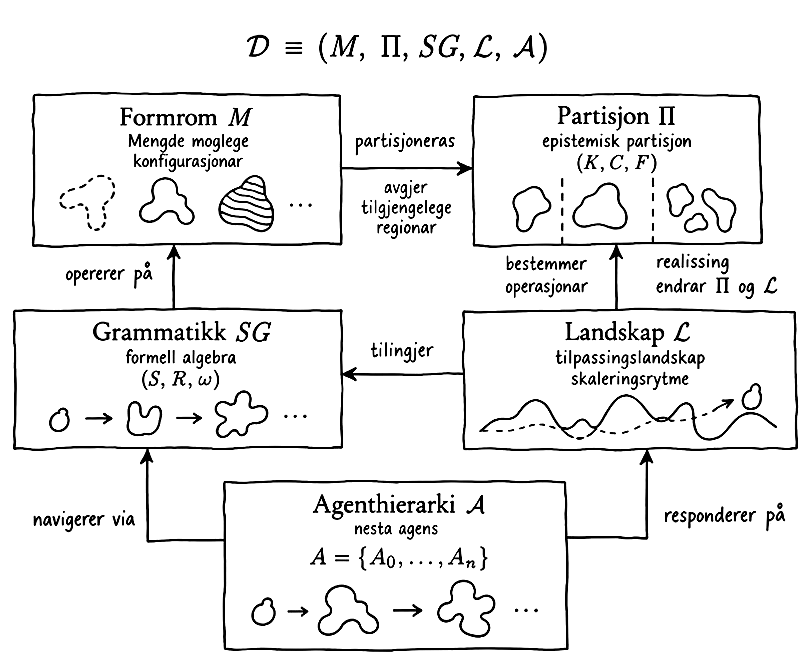
\includegraphics[width=\linewidth]{scan-20261031-p35-d-modell-diagram.png}
\caption{Formrom, grammatikk, landskap og agentar}
\end{figure}

\prop{6.67}{d}{Den samla omhugen langs X\textsubscript{k} er W\textsubscript{k} = \ensuremath{∑}\textsubscript{i} w\textsubscript{i} \ensuremath{ω}\textsubscript{k}(A\textsubscript{i}), rekna over dei agentane som held aksen.}

\prop{6.671}{t}{Der W\textsubscript{k} = 0, vel ingen langs aksen.

Gjeve koordinatane x\textsubscript{H} langs dei haldne aksane, er fordelinga langs aksen grammatikken si eiga, avgrensa til det som ikkje er forbode:

\formel{P(x_{k} | x_{H}) = μ_{SG}(x_{k} | x_{H}, x ∉ V)}

Der er forma berre det moglege, ikkje det valde. Ho fell der ho fell.}

\prop{6.672}{t}{Langs ein akse er variansen nær ein dalbotn omvendt proporsjonal med kor krapp dalen er og kor mykje samla omhug som verkar langs aksen: Var(xk ) \ensuremath{≈} 1/(\ensuremath{β} Wk \ensuremath{\hat{\Lambda}}\ensuremath{′}\ensuremath{′}k ), der \ensuremath{\hat{\Lambda}}\ensuremath{′}\ensuremath{′}k er krumminga langs Xk i dalbotnen. Tilnærminga gjeld når spenninga lèt seg dele akse for akse, agentane er samde om krumminga, og grunnfordelinga er flat nær botnen.

Kanaliseringa (3.2) og omhugen er då to sider av same spreiing.}

\prop{6.6721}{i}{Tenk ei samling stolar der variasjonskoeffisienten er 0,07 for setehøgda og 1,5 for ornamentet. Tala er illustrasjonstal. Modellen ville lese skilnaden slik: kroppen held setehøgda; ingen held ornamentet like fast.}

\prop{6.68}{t}{Forma vert vald i det landskapet agentane estimerer langs det dei held, men ho står (6.611) i det landskapet som er.}

\mainprop{7}{t}{Forma viser kor langt omhugen rakk.}

\prop{7.01}{t}{Kvar realisert form er eksakt langs alle aksar (1.12, 1.32), og aksane tek ikkje slutt (1.322). Kvar agent held endeleg mange (5.1141), og ei form vert navigert av endeleg mange agentar.

Forma rekk difor alltid lenger enn den samla omhugen.}

\prop{7.02}{t}{Langs dei aksane nokon heldt (6.67), er forma vald. Langs dei andre fell ho der ho fell (6.671), innanfor det grammatikken og substratet tillèt.

Over mange former sett er mønsteret av det valde og det uvalde (6.672) eit kart over den samla omhugen.}

\prop{7.021}{t}{Omhug utan kapasitet rakk ikkje fram til forma (5.232). Det forma viser, kor langt omhugen rakk fram, er ikkje heile lyskjegla, men dei haldne aksane (5.231).}

\prop{7.03}{t}{Forma er utfallet av politikkane som navigerte henne (6.64). Der ein politikk set arbeid i gang mot avvik, er han omhug, sett utanfrå (5.261).

Langs dei haldne aksane er forma difor omhug, sett utanfrå; langs dei andre (7.02) fell ho berre.}

\prop{7.031}{t}{Materie er oppleving, sett utanfrå (1.2351). Det levande er eit sjølv, sett utanfrå (5.62).

Forma er omhug, sett utanfrå, så langt omhugen rakk.}

\prop{7.04}{t}{Omhugen ein gjenstand viser, er lånt: omhugen til dei som forma han, festa i materialet. Gjenstanden held ikkje si eiga hinne (5.023); han har inga eiga innside.}

\prop{7.041}{t}{Gjenstanden er difor eit arkiv. Han ber omhug som ingen lenger held.}

\prop{7.1}{t}{Den realiserte forma er eit leseleg arkiv over dimensjonaliteten i kompromisset.

Ei form designa under trong omhug sviktar, sett over mange former, langs dei aksane som ikkje vart haldne og der trykk verkar, for trykka der verkar framleis (5.2321, 6.68).

Kvar svikten kjem, er ikkje tilfeldig. Svikten ber signaturen av det som produserte han: blindskapen, likesæla eller avmakta (5.232).}

\prop{7.11}{t}{Signaturen er leseleg fordi skiljet mellom det valde og det uvalde ikkje er tilfeldig.

Skiljet følgjer grensa for det agentane heldt. Forma er residuet av ein retta prosess.

Retninga er gjeven av gradienten i estimata (6.611); kva aksar ho rører, av det agentane held (5.231).}

\prop{7.12}{t}{Former designa under ulik omhug for same funksjon skil seg, sett over mange, systematisk langs dei aksane den eine sida heldt og den andre ikkje.

Skilnaden er arkivet.}

\prop{7.13}{t}{Arkivet er ikkje ei skulding, men eit faktum. (Same faktumet som gjer \hyperlink{kjeldenotat-7.13}{geologi leseleg}, gjer design leseleg\kjelde{72}.)}

\prop{7.14}{d}{Kor mange horisontar svikten ventar, er sviktlatensen: \ensuremath{ρ}k (A) = \ensuremath{Δ}k / \ensuremath{τ}k (A), der \ensuremath{Δ}k er tida før konsekvensen viser seg langs Xk, og \ensuremath{τ}k (A) er horisonten langs aksen (5.114).}

\prop{7.141}{d}{Forholdstalet deler svikten i tre regime:

\ensuremath{ρ} \ensuremath{≤} 0,1 · Internalisert: konsekvensen ligg godt innanfor horisonten; svikten kan føreseiast innanfrå.\\
0,1 < \ensuremath{ρ} < 100 · Leseleg: konsekvensen kjem nær horisonten, eller høgst to storleiksordenar etter han, så signaturen kan observerast.\\
\ensuremath{ρ} \ensuremath{≥} 100 · Strukturelt usynleg: konsekvensen kjem storleiksordenar etter horisonten; agenten kan ikkje lese signaturen utan ekstern representasjon.}

\prop{7.142}{i}{To tenkte rekneeksempel.

Ergonomi: set horisonten i prøvesitjinga til éin time og tida før ryggverken til åtte timar; \ensuremath{ρ} = 8, leseleg.

Eingongskoppen: set brukshorisonten til tjue minutt og nedbrytingstida til fire hundre år; \ensuremath{ρ} \ensuremath{∼} 10\textsuperscript{7}, strukturelt usynleg.

Same formalisme; ulikt forholdstal.}

\begin{figure}[htbp]\centering
\includegraphics[width=\linewidth]{scan-20261031-p41-sommarfugl-livslop.png}
\caption{Larve, puppe og sommarfugl}
\end{figure}

\prop{7.143}{t}{Utanfor kapasiteten er horisonten null og sviktlatensen uendeleg. Svikten kan altså ikkje sjåast kome.

Blindskapen kan ikkje lese sin eigen signatur, for aksen set han ikkje i spenning (5.262).

Avmakta kjenner svikten som uro når han kjem (5.2611), men kan ikkje sjå han kome.

Likesæla kunne sjå han kome; ho gjer det ikkje.}

\prop{7.144}{t}{Sviktlatensen er relativ til den som les. Ein signatur som er usynleg for den som formgav, kan vere leseleg (1.531) for ein observatør med aksen i lyskjegla si og ein lengre horisont.}

\prop{7.15}{t}{\hyperlink{kjeldenotat-7.15}{Sviktsignatur} kan ikkje predikerast av ein designteori utan omgrep om omhug, lyskjegle og kapasitet. Ein slik teori kan berre registrere signaturen i ettertid.}

\prop{7.151}{t}{Prediksjonen krev at teorien namngjev grensa for det agentane held.

Prediksjonen krev ikkje at landskapet er lodda, for det lèt seg berre lodde i ettertid (3.11). Han krev landskapet ikkje som kart, men som omgrep: at trykk verkar vidare langs aksar ingen held (5.2321).

Utan grensa finst ingen akse å peike ut som uhalden før svikten kjem.}

\prop{7.152}{t}{Svikt er spenning i det verkelege landskapet, langs aksar omhugen ikkje rakk, i former grammatikken kunne generere.

Grammatikken åleine (5.72 i) veit kva som kan bli, ikkje kva som vil svikte.

Tanke-kunnskapsteorien åleine (5.72 ii) veit kva som er kjent, ikkje kvar det ukjende vil slå til.

Optimeringa åleine (5.72 iii) skjerper dei aksane ho har, og er blind for resten.

Prediksjon krev difor alle dei tre laga som omgrep, men ikkje eit ferdig kart over landskapet.}

\prop{7.1521}{t}{Berre den allvitande agenten (5.72 iv) ville ikkje etterlate nokon signatur av det uhaldne. Det som stod att, ville vere kompromisset sjølv (2.131).

Men grensetilfellet (iv) er ein horisont (5.7221), ikkje ein stad.}

\prop{7.153}{t}{Å forklare ei form er å forklare kvifor dei andre ikkje vart realiserte (1.131). Langs aksar ingen heldt, vart dei ikkje utelukka av noko val (7.02).

Ein teori som ikkje skil desse aksane frå dei andre, kan ikkje predikere sviktsignatur (7.151). Han forklarer ikkje form, men katalogiserer henne.

Sviktsignaturen er såleis ikkje ein empirisk bonus, men prøvesteinen på at teorien forklarer form.}

\prop{7.16}{t}{Læra i 5.521, trong omhug gjord til program, er det reinaste dømet. Formene hennar ber signaturen til læra.}

\prop{7.2}{t}{Designhandlinga verkar inn på dei generative modellane til andre agentar, langs dei aksane der kriteriet i 6.02 er oppfylt.

Dette er ein påstand om verknad, ikkje om verdi. Kva som følgjer av han, avheng av vurderingsapparatet til agenten sjølv.}

\prop{7.201}{t}{Ein verknad på modellen til eit sjølv er, innanfrå, ein verknad på kva det kjenner (5.2611). Påstanden er framleis deskriptiv.}

\prop{7.21}{t}{Langs kvar akse ingen heldt, bar ingen avviket då forma vart til. Får nokon aksen i lyskjegla si seinare, ber han avviket utan dei som forma henne (6.027).

Det som utanfrå er ein sviktsignatur, er altså innanfrå uro (5.2611) hjå den som lever med forma, så lenge han ikkje kan halde aksen (5.232).}

\prop{7.22}{t}{Der sviktsignaturen råkar eit sjølv, er han uroa til den som ikkje var med, sett utanfrå.}

\prop{7.23}{d}{Mengda av aksar i \ensuremath{𝕄} som ingen agent held, slik at Wk = 0, og der trykk verkar, er det predikerte sviktrommet.

Kvar av aksane har sviktlatensen \ensuremath{ρ}k (A) for den agenten A som les. For kvar agent fell det predikerte sviktrommet i tre: blindskap, likesæle og avmakt (5.232).

Formmodellen predikerer at forma ber signatur langs desse aksane.

Om signaturen er relevant for agenten, er ikkje eit spørsmål modellen svarar på, men eit spørsmål agenten stiller når han les modellen.}

\prop{7.24}{t}{Modellen kan ikkje måle at noko har noko å seie.

Målingane hans er relasjonar (1.2311), og det å ha noko å seie er innsida av det han skildrar utanfrå (5.261).

Han kan berre vise kvar noko hadde noko å seie for nokon som kunne halde det, og kvar ikkje.}

\prop{7.25}{t}{Omhugen veit ikkje sjølv kor langt han rakk fram, for grensa hans er usynleg innanfrå (5.263). Sløyfa vert lukka utanfrå: av svaret frå den som tok imot, eller av ein annan (7.144) som les forma.}

\prop{7.3}{t}{Desse proposisjonane er sjølve ei form.

\hyperlink{kjeldenotat-7.3}{Dei er ein stige}, navigert steg for steg av ein agent med endeleg horisont (5.1142) og endeleg mange (7.01) haldne aksar.}

\prop{7.31}{t}{Proposisjonane sviktar difor langs aksar eg ikkje heldt (7.1).

Somme av aksane kunne eg nemne, for ein kan sjå ein akse og likevel ikkje halde han (5.232).

Det som låg utanfor det eg kunne tenkje, kan ikkje nemnast her, for den grensa (1.53, 5.263) er usynleg innanfrå.}

\prop{7.32}{t}{Ein lesar som held aksar eg ikkje heldt, kan lese signaturen til proposisjonane (7.144) og sjå kvar stega ikkje bar. Lesinga hans er svaret (7.25) som lukkar sløyfa.}

\prop{7.33}{t}{\hyperlink{kjeldenotat-7.33}{Stigen vert difor ikkje kasta}. Utanfor feltet finst det inkje å stige opp til (1.246).

Han vert lesen.}

\prop{7.34}{t}{Fjellet er ikkje i kartet. Men den som les kartet (1.3211), står på fjellet.}

\prop{7.4}{t}{\hyperlink{kjeldenotat-7.4}{Formverda er alt som er tilfelle}, og alt som er tilfelle, verkar. Navigasjonen held fram.}
